\documentclass[
  language=english,
  thesis=bachelor,
  faculty=cb,
  nosecondtitle,
  onesided,
  compactlistof,
  fancy,
  open=any
]{hsmw-thesis}

\title{Statistical Drift Detection for Non-Stationary Black-Box LLM Classifiers}
\author{Georgii}{Burdin}
\submissiondate{2026}[08][14]
\courseofstudy{B.Sc. Applied Mathematics}
\seminargroup{MA22w1-B}
\examiner[Prof.\ Dr.\ rer.\ nat.\ Dr.-Ing.\ habil.]{Florian Zaussinger}
\addexaminer[M.Sc.]{Marin Ivankovic}[Co-Founder \& CEO of GOCOMO GmbH]
\abstract{%
This thesis investigates how black-box Large Language Model classifiers used for campaign-relevance detection can be monitored over time and evaluated for deployment when their behaviour may change without notice. It combines repeated evaluation on a fixed sentinel panel with exact paired statistical testing, multiplicity control, and a separate cost-aware comparison of deployment candidates. The approach is implemented as a reproducible batch workflow that preserves item-level outputs and run identity for later analysis. The empirical study shows that the framework can identify a meaningful change in observed model behaviour, while distinguishing such an alert from evidence about its cause or production impact. It further demonstrates that model selection depends on both classification errors and inference cost rather than accuracy alone. Overall, the thesis provides an auditable decision process connecting monitoring, statistical escalation, and deployment selection.
}
\email{\href{mailto:gburdin@hs-mittweida.de}{gburdin@hs-mittweida.de}}
\location{Mittweida}
\date{\today}


%%%%%%%%%%%%%%%%%%%%%%%%%%%%%%%%%%%%%%%%%%
%%% Bibliography
\usepackage[bibstyle=ieee,citestyle=numeric-comp,natbib=true,sorting=none,dashed=false]{biblatex}
\usepackage{xcolor}
\usepackage{bm}
\usepackage{listings}
\usepackage{graphicx}
\usepackage{xurl}
\usepackage{tikz}
\usetikzlibrary{positioning,arrows.meta,calc,fit,shapes.geometric,backgrounds}
\usepackage{pgfplots}
\pgfplotsset{compat=1.18}

% Let TeX stretch spacing in hard paragraphs instead of running into the margin.
% The chapters are dense with unbreakable \texttt{} identifiers and file paths.
\setlength{\emergencystretch}{3em}

% Figure palette (validated categorical slots 1-2 plus chrome greys).
\definecolor{vizblue}{HTML}{2A78D6}
\definecolor{vizorange}{HTML}{EB6834}
\definecolor{vizgrid}{HTML}{E1E0D9}
\definecolor{vizaxis}{HTML}{C3C2B7}
\definecolor{vizmuted}{HTML}{898781}
\definecolor{vizink}{HTML}{52514E}
\usepackage[edges]{forest}
\usepackage{float}
\usepackage{placeins}
\usepackage{adjustbox}
% Preamble
\usepackage{booktabs}
\usepackage{tabularx}
\usepackage{ragged2e}
\usepackage{array}
\captionsetup{font=small,labelfont=bf,skip=0.4\baselineskip}



\tikzset{
  figbox/.style={
    draw,
    rectangle,
    rounded corners=1pt,
    align=center,
    font=\footnotesize,
    minimum height=8mm,
    text width=25mm,
    inner sep=3pt
  },
  figboxsmall/.style={
    draw,
    rectangle,
    rounded corners=1pt,
    align=center,
    font=\scriptsize,
    minimum height=7mm,
    text width=17mm,
    inner sep=2pt
  },
  figarrow/.style={
    ->,
    thick,
    >=Latex
  },
  figdiamond/.style={
    draw,
    diamond,
    aspect=2.4,
    align=center,
    font=\footnotesize,
    inner sep=1pt,
    minimum width=22mm,
    minimum height=11mm
  }
}
% already loaded above with 'fit'

\addbibresource{literature.bib}

% Theorem-style environments used in the formalisation
\theoremstyle{plain}
\newtheorem{assumption}{Assumption}
\newtheorem{proposition}{Proposition}
\newcolumntype{L}[1]{>{\RaggedRight\arraybackslash}p{#1}}
\newcolumntype{Y}{>{\RaggedRight\arraybackslash}X}

% Keep the main contents at thesis-outline level; derivation signposts remain in the body.
\setcounter{tocdepth}{1}
\RedeclareSectionCommand[tocbeforeskip=0pt]{chapter}
\BeforeStartingTOC[toc]{\small}

% Auto-generated — 2026-03-28
% Usage: \csname benchgpt41miniaccuracy\endcsname (digits in names require \csname)
\expandafter\newcommand\csname benchgpt41miniaccuracy\endcsname{0.799331}
\expandafter\newcommand\csname benchgpt41miniprecision\endcsname{0.994764}
\expandafter\newcommand\csname benchgpt41minirecall\endcsname{0.763052}
\expandafter\newcommand\csname benchgpt41minif1\endcsname{0.863636}
\expandafter\newcommand\csname benchgpt41minispecificity\endcsname{0.980000}
\expandafter\newcommand\csname benchgpt41minibalancedaccuracy\endcsname{0.871526}
\expandafter\newcommand\csname benchgpt41miniprauc\endcsname{0.977571}
\expandafter\newcommand\csname benchgpt41nanoaccuracy\endcsname{0.733333}
\expandafter\newcommand\csname benchgpt41nanoprecision\endcsname{0.956989}
\expandafter\newcommand\csname benchgpt41nanorecall\endcsname{0.712000}
\expandafter\newcommand\csname benchgpt41nanof1\endcsname{0.816514}
\expandafter\newcommand\csname benchgpt41nanospecificity\endcsname{0.840000}
\expandafter\newcommand\csname benchgpt41nanobalancedaccuracy\endcsname{0.776000}
\expandafter\newcommand\csname benchgpt41nanoprauc\endcsname{0.954495}

% Generated by scripts/sync_canonical_evidence.py; do not edit.
\providecommand{\CanonicalVersion}{canonical-evidence-v1.0.0}
\providecommand{\CanonicalRuns}{187}
\providecommand{\CanonicalModels}{12}
\providecommand{\CanonicalComparisons}{173}
\providecommand{\CanonicalRawSignificant}{3}
\providecommand{\CanonicalHolmAlerts}{1}
\providecommand{\CanonicalAlertPairs}{296}
\providecommand{\CanonicalAlertB}{49}
\providecommand{\CanonicalAlertC}{12}
\providecommand{\CanonicalAlertDrop}{12.5}
\providecommand{\CanonicalCostN}{1112}
\providecommand{\CanonicalCostWinner}{\texttt{gpt-5-mini}}


\newsavebox{\PayloadListingBox}

\begin{document}

% 00_company_approval_statement.tex is signed separately and bound in by hand.

\chapter{Introduction}

\section{Context and motivation}
Industrial classification pipelines increasingly rely on Large Language Model providers that expose their systems through application programming interfaces. In such settings, the deployed model can be viewed as a non-stationary black-box classifier whose internal parameters and update schedule are controlled by the provider rather than by the user. As a result, the behaviour of the same API-accessible model may change over time even when the task, prompt, and evaluation procedure remain fixed~\cite{chen2023chatgpt,openai2026modelguidance,anthropic2026modelversioning}.

The practical motivation for this thesis arises from the author's work at GOCOMO GmbH. In the company's social-media analytics workflow, LLMs are used in batch mode to determine whether a post is relevant to a specified campaign, brand, or event. This is naturally formulated as a binary classification task. Because the volume of incoming content is large, automated classification becomes a necessary operational component.

However, the use of external LLM APIs creates a reliability problem. A model that performs well during an initial benchmark may later degrade after a provider-side change~\cite{chen2023chatgpt,openai2026modelguidance,anthropic2026modelversioning}. In a business-critical pipeline, such changes should be detected early. At the same time, repeated full-benchmark evaluation on a labelled dataset is costly. This creates the need for a monitoring procedure that is statistically informative, operationally feasible, and economically justified.

\section{Task definition and request contract}
GOCOMO uses closed LLM APIs to classify social-media posts as relevant or not relevant to a marketing campaign. These predictions are used to filter content before downstream analytics. Because the incoming volume is large, the decision has to be made automatically and then checked through offline evaluation rather than routine manual review.

The task is semantic rather than a keyword lookup. A post can refer to a campaign through its text, visuals, or context without repeating a campaign name or hashtag. The main difficulty is that many posts are topically similar to campaign content while still lacking a direct connection to the campaign itself.

Figure~\ref{fig:campaign-relevance-examples} shows the intended distinction. The relevant post is linked to the GOCOMO Effie event through the submission materials and the workspace context. The non-relevant post shows branded merchandise only, without an event connection.

\begin{figure}[htbp]
\centering
\begin{adjustbox}{max width=\linewidth}
\begin{tikzpicture}[
    >=Latex,
    frame/.style={draw=vizaxis, line width=0.5pt, rounded corners=1.5pt, fill=white, inner sep=4.5pt},
    panel/.style={draw=vizaxis, line width=0.5pt, rounded corners=1.5pt, fill=vizgrid!14, align=left, inner sep=5.5pt},
    badge/.style={rounded corners=1.5pt, inner sep=3.2pt, font=\scriptsize\bfseries},
    callout/.style={draw=vizblue, fill=vizblue!12, rounded corners=1pt, inner sep=2.2pt, font=\tiny\bfseries, text=vizink}
]
% Campaign brief
\node[panel, text width=0.97\linewidth] (campaign) {%
  \textbf{Campaign:} GOCOMO Effie event\quad
  {\scriptsize A post is relevant only if it is clearly linked to the Effie event itself.}
};

% Post A - relevant
\node[frame, below=5.5mm of campaign.south west, anchor=north west, text width=0.455\linewidth] (posta) {%
  \textbf{Post A}\\[2.5pt]
  
\includegraphics[width=\linewidth]{assets/examples/thumb_relevant.png}\\[3.5pt]
  {\scriptsize\texttt{"Finalising the Effie report."}}\\[3pt]
  {\scriptsize\textbf{Evidence}}\\[0.5pt]
  {\scriptsize
  \begin{itemize}\setlength\itemsep{0.4pt}\setlength\parsep{0pt}\setlength\topsep{1pt}\setlength\leftmargini{1.1em}
  \item Effie submission materials on screen
  \item GOCOMO mug visible in the workspace
  \item explicit event-related context
  \end{itemize}}
};

% Post B - not relevant
\node[frame, below=5.5mm of campaign.south east, anchor=north east, text width=0.455\linewidth] (postb) {%
  \textbf{Post B}\\[2.5pt]
  
\includegraphics[width=\linewidth]{assets/examples/thumb_not_relevant.png}\\[3.5pt]
  {\scriptsize\texttt{"I love my merch."}}\\[3pt]
  {\scriptsize\textbf{Evidence}}\\[0.5pt]
  {\scriptsize
  \begin{itemize}\setlength\itemsep{0.4pt}\setlength\parsep{0pt}\setlength\topsep{1pt}\setlength\leftmargini{1.1em}
  \item branded mug visible
  \item brand merchandise only
  \item no Effie event link
  \end{itemize}}
};

% Callouts constrained to Post A only
\begin{scope}
\node[callout] (eventcall) at ($(posta.north)+( -0.55cm,-1.45cm)$) {Effie report};
\draw[->, draw=vizblue, line width=0.55pt] (eventcall.south) -- ++(0,-0.42);
\node[callout] (mugcall) at ($(posta.north east)+(-1.35cm,-2.35cm)$) {GOCOMO mug};
\draw[->, draw=vizblue, line width=0.55pt] (mugcall.south) -- ++(0,-0.42);
\end{scope}

\node[badge, fill=vizblue!16, draw=vizblue, below=2.8mm of posta] {Decision: Relevant};
\node[badge, fill=vizorange!18, draw=vizorange, below=2.8mm of postb] {Decision: Not relevant};
\end{tikzpicture}

\end{adjustbox}
\caption[Representative campaign-relevance examples]{Representative examples of the binary decision. Relevance requires an explicit link to the Effie event.}
\label{fig:campaign-relevance-examples}
\end{figure}

In the formal chapters, the observed output for post \(x_i\) at time \(t\) is written as
\[
\hat y_{i,t}(q)=Q(x_i;c_t,h_t)=q_t(x_i).
\]
This notation separates the client-controlled request contract \(c_t\) from the hidden provider-side state \(h_t\). The contract includes the prompt, request schema, parser, and any exposed inference settings that are available for the chosen model. The hidden state includes inaccessible weights, routing, and the remaining server-side execution behaviour. The classifier is therefore observed only through its outputs over time.

For every post, the request combines a campaign brief with caption, transcript, hashtags, mentions, metadata, and selected images or video frames. The strict output schema requires \texttt{campaign\_relevant:boolean} and \texttt{relevancy\_reasoning:string}; only the boolean enters the metrics. Figure~\ref{fig:payload-unified} shows the canonical contract before provider-specific adaptation.

\begin{figure}[H]
\centering
\begin{adjustbox}{max width=\linewidth}
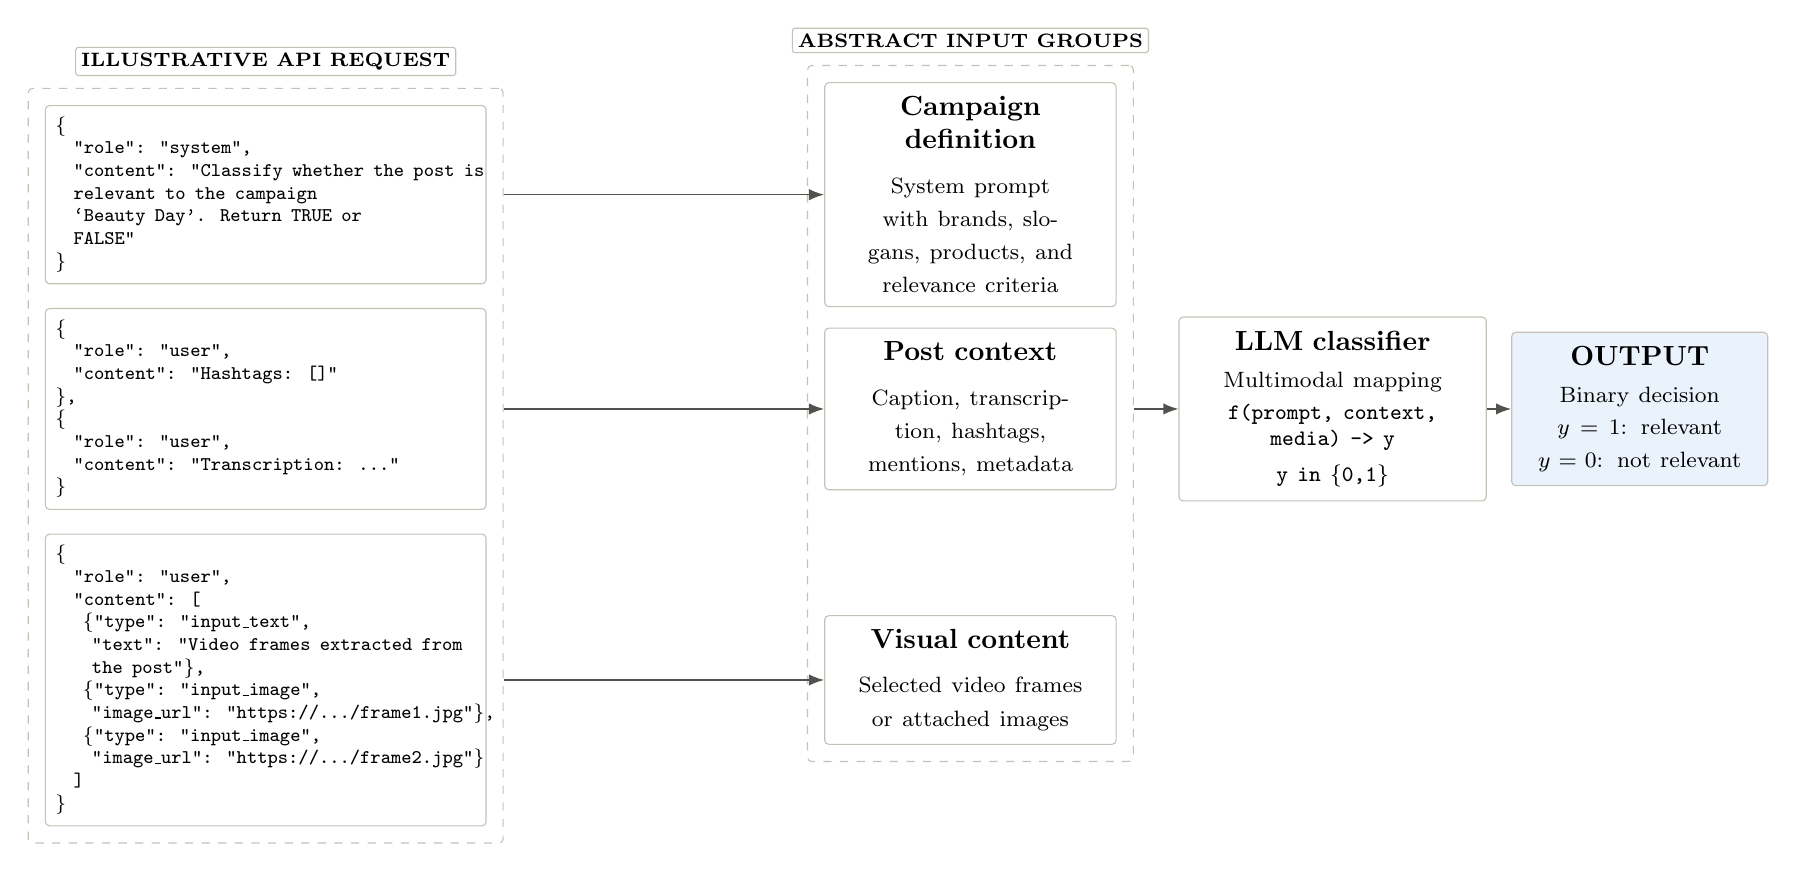
\begin{tikzpicture}[
    >=Latex,
    msgbox/.style={draw=vizaxis, rounded corners=1.5pt, align=left,
        text width=5.35cm, inner sep=3.5pt, fill=white},
    groupframe/.style={draw=vizaxis, dashed, rounded corners=1.5pt, inner sep=5pt},
    groupbox/.style={draw=vizaxis, rounded corners=1.5pt, align=center,
        text width=3.35cm, minimum height=16mm, inner sep=5pt, fill=white},
    modelbox/.style={draw=vizaxis, rounded corners=1.5pt, align=center,
        text width=3.55cm, minimum height=20mm, inner sep=5pt, fill=white},
    outputbox/.style={draw=vizaxis, rounded corners=1.5pt, align=center,
        text width=2.9cm, minimum height=16mm, inner sep=5pt, fill=vizblue!10},
    tag/.style={draw=vizaxis, rounded corners=1pt, fill=white, inner sep=2pt, font=\scriptsize\bfseries},
    flow/.style={->, line width=0.55pt, draw=vizink}
]
% Three payload slices, stacked then mirrored by the three abstract groups
\node[msgbox] (msgcamp) {%
\ttfamily\fontsize{7}{8.2}\selectfont
\begin{tabular}{@{}l@{}}
\{ \\
\ \ "role": "system", \\
\ \ "content": "Classify whether the post is \\
\ \ relevant to the campaign \\
\ \ `Beauty Day'. Return TRUE or \\
\ \ FALSE" \\
\}
\end{tabular}};
\node[msgbox, below=3mm of msgcamp] (msgctx) {%
\ttfamily\fontsize{7}{8.2}\selectfont
\begin{tabular}{@{}l@{}}
\{ \\
\ \ "role": "user", \\
\ \ "content": "Hashtags: []" \\
\}, \\
\{ \\
\ \ "role": "user", \\
\ \ "content": "Transcription: ..." \\
\}
\end{tabular}};
\node[msgbox, below=3mm of msgctx] (msgvis) {%
\ttfamily\fontsize{7}{8.2}\selectfont
\begin{tabular}{@{}l@{}}
\{ \\
\ \ "role": "user", \\
\ \ "content": [ \\
\ \ \ \{"type": "input\_text", \\
\ \ \ \ "text": "Video frames extracted from \\
\ \ \ \ the post"\}, \\
\ \ \ \{"type": "input\_image", \\
\ \ \ \ "image\_url": "https://.../frame1.jpg"\}, \\
\ \ \ \{"type": "input\_image", \\
\ \ \ \ "image\_url": "https://.../frame2.jpg"\} \\
\ \ ] \\
\}
\end{tabular}};
\node[groupframe, fit=(msgcamp)(msgctx)(msgvis), inner sep=6pt] (requestframe) {};
\node[tag, anchor=south] at ($(requestframe.north)+(0,1.5mm)$) {ILLUSTRATIVE API REQUEST};

\node[groupbox] (campaign) at (8.95,0 |- msgcamp) {%
  \textbf{\normalsize Campaign definition}\\[4pt]
  \footnotesize System prompt with brands, slogans, products, and relevance criteria};
\node[groupbox] (context) at (8.95,0 |- msgctx) {%
  \textbf{\normalsize Post context}\\[4pt]
  \footnotesize Caption, transcription, hashtags, mentions, metadata};
\node[groupbox] (visual) at (8.95,0 |- msgvis) {%
  \textbf{\normalsize Visual content}\\[4pt]
  \footnotesize Selected video frames or attached images};
\node[groupframe, fit=(campaign)(context)(visual), inner sep=6pt] (groupframe) {};
\node[tag, anchor=south] at ($(groupframe.north)+(0,1.5mm)$) {ABSTRACT INPUT GROUPS};

\node[modelbox] (model) at (13.55,0 |- msgctx) {%
  \textbf{\normalsize LLM classifier}\\[4pt]
  \footnotesize Multimodal mapping\\[2pt]
  \footnotesize\texttt{f(prompt, context, media) -> y}\\[1pt]
  \footnotesize\texttt{y in \{0,1\}}};
\node[outputbox] (output) at (17.45,0 |- msgctx) {%
  \textbf{\normalsize OUTPUT}\\[4pt]
  \footnotesize Binary decision\\[2pt]
  \footnotesize $y=1$: relevant\\$y=0$: not relevant};

% Left: three parallel horizontals. Right: one trunk, no fan-in.
\draw[flow] (msgcamp.east -| requestframe.east) -- (campaign.west);
\draw[flow] (msgctx.east -| requestframe.east) -- (context.west);
\draw[flow] (msgvis.east -| requestframe.east) -- (visual.west);
\draw[flow] (groupframe.east |- model.west) -- (model.west);
\draw[flow] (model.east) -- (output.west);
\end{tikzpicture}
\end{adjustbox}
\caption[Unified representation of the multimodal classification request]{Unified representation of the multimodal classification request. The left side shows an illustrative provider-facing API payload. The right side abstracts the same request into three conceptual input groups: campaign definition, post context, and visual content. The arrows indicate how payload components map to the inputs of the classifier, which returns a binary relevance decision.}
\label{fig:payload-unified}
\end{figure}

These task and request definitions fix the observable object used throughout the thesis: a repeated black-box binary decision on the same labelled items under a fixed client-controlled request contract. If the prompt or another exposed request component is intentionally changed, that is treated as a new configuration rather than passive drift of the old one.

\section{Problem statement and research questions}
The central problem is to evaluate and monitor API-based LLM classifiers in a production environment where model behaviour may change over time. The user does not control the underlying model updates, yet still has to make reliable decisions from observed task performance.

The thesis addresses this problem through four research questions:
\begin{enumerate}
    \item[RQ1:] How can campaign-relevance classification by an external LLM API be formalised as repeated evaluation of a non-stationary black-box binary classifier?
    \item[RQ2:] How can a reduced monitoring subset be constructed and sized so that routine evaluation is substantially cheaper while retaining sensitivity to behavioural change?
    \item[RQ3:] Which paired statistical test and multiplicity treatment provide an appropriate rule for detecting directional degradation across repeated runs?
    \item[RQ4:] How should candidate models be compared and selected when predictive quality, inference cost, and campaign-specific false-positive and false-negative costs differ?
\end{enumerate}

\section{Structure}
The thesis is organised as follows:
\begin{itemize}
    \item Chapter~\ref{ch:data} defines the benchmark and sensitivity panel.
    \item Chapter~\ref{ch:drift} derives the paired monitoring test and its scope.
    \item Chapter~\ref{ch:cost-deployment-utility} defines a separate cost-aware decision rule.
    \item Chapter~\ref{chap:system-architecture} describes the implementation.
    \item Chapter~\ref{chap:experimental-results} reports the recorded episode and candidate comparison.
    \item Chapter~\ref{chap:conclusion} summarises the main findings and limitations.
\end{itemize}
The appendix presents automatic prompt optimisation as an exploratory drift-mitigation extension: prompt repair can provide a practical recovery path alongside model switching when drift is detected, although its effect remains episode-dependent and requires the same full re-evaluation protocol.


\chapter{Data and Evaluation Setup}

\section{Formal Problem Definition}
To evaluate model drift rigorously, we must first define the classification task within a probabilistic framework. Let $\mathcal{X} \subset \mathbb{R}^d$ denote the high-dimensional input space of social-media posts (comprising text, metadata, and visual features) and $\mathcal{Y} = \{0, 1\}$ the binary label space, where $1$ indicates relevance to a campaign. 

In the context of LLM-as-a-Service, the model is a non-stationary black box. We define the classifier as a function $f(x; \pi, \theta_t) \to \hat{y} \in \{0, 1\}$, where $\pi$ is a fixed prompt and $\theta_t$ represents the hidden, time-varying model weights. 

Under the zero-one loss function $\mathcal{L}(\hat{y}, y) = \mathbb{I}(\hat{y} \neq y)$, the \textbf{Expected Risk} (or true error rate) at time $t$ is:
\begin{equation}
    R_t(f) = \mathbb{E}_{(x,y) \sim P_t} [\mathbb{I}(f(x; \pi, \theta_t) \neq y)]
\end{equation}
Since the true data-generating distribution $P_t$ is unknown, we must estimate this risk empirically.

\section{The Reference Benchmark vs. Operational Constraints}
Let $\mathcal{D}_N$ be the reference benchmark consisting of $N = 1199$ manually labelled examples, establishing the ground truth. Evaluating all candidate models against $\mathcal{D}_N$ yields a highly precise empirical risk $\hat{R}_N$. 

However, running inference on $N=1199$ instances weekly across multiple candidate models is economically prohibitive. We require a monitoring subset $\mathcal{D}_n \subset \mathcal{D}_N$ of size $n \ll N$. The central mathematical challenge is to select $\mathcal{D}_n$ such that it remains highly sensitive to temporal shifts in the parameters $\theta_t$, despite the significantly reduced sample size.

\section{Reference benchmark and monitoring subset}
\label{sec:input-datasets}

The two sets $\mathcal{D}_N$ and $\mathcal{D}_n$ are stored as fixed Langfuse datasets sharing one schema and label column (\texttt{campaign\_relevant}). Table~\ref{tab:dataset-summary} summarises their composition.

\begin{table}[htbp]
    \centering
    \caption{Full reference benchmark (\texttt{campaign\_relevance\_02e1a68ccb0f}) and monitoring subset (\texttt{campaign\_relevance\_disagree\_subset\_9d488308aa46}): size, class balance, and modality composition.}
    \label{tab:dataset-summary}
    \begin{tabular}{lcc}
        \toprule
        & \textbf{Full benchmark} & \textbf{Monitoring subset} \\
        \midrule
        Number of posts ($N$ / $n$) & 1199 & 300 \\
        Relevant (\texttt{campaign\_relevant}${}=1$) & 682 (56.9\%) & 250 (83.3\%) \\
        Not relevant (\texttt{campaign\_relevant}${}=0$) & 517 (43.1\%) & 50 (16.7\%) \\
        Image posts & 288 & 78 \\
        Video posts & 911 & 222 \\
        Total attached images (all posts) & 5911 & 1762 \\
        Mean images per post & 4.93 & 5.87 \\
        \bottomrule
    \end{tabular}
\end{table}

Each post is tagged as an \textbf{image post} (one image) or a \textbf{video post} (several frames). Both sets are \textbf{class-imbalanced}; the subset is far more positive-heavy than $\mathcal{D}_N$ (Table~\ref{tab:dataset-summary}), which follows from disagreement-based construction (Section~\ref{sec:informative-sampling-disagreement}). Accuracy figures on $\mathcal{D}_N$ and $\mathcal{D}_n$ are not interchangeable---prevalence differs, not only sample size.

Roughly three quarters of items are \textbf{video posts} in both splits; multi-frame requests carry more multimodal tokens than single-image ones. The subset is not a stratified copy of the full benchmark: it has a slightly larger fraction of image posts (78/300 vs.\ 288/1199) but still a \textbf{higher} mean images per post (5.87 vs.\ 4.93), so monitored runs are visually heavier and costlier to repeat. Subsequent empirical sections report metrics on $\mathcal{D}_n$ only; they characterise model behaviour on this fixed disagreement subset, not a simple random replicate of $\mathcal{D}_N$'s label prevalence or its image--video mix.

\section{Informative Sampling via Model Disagreement}
\label{sec:informative-sampling-disagreement}
A simple random sample (SRS) of size $n$ would yield an unbiased estimator of $R_t$. However, the vast majority of social-media posts are "easy" instances located far from the model's decision boundary, where the conditional probability $P(Y=1|X) \approx 1$ or $0$. These instances exhibit low prediction variance and are highly robust to small parameter shifts in $\theta_t$. 

To maximize the sensitivity of our monitoring subset, we abandon uniform sampling in favor of \textbf{Uncertainty Sampling}. We construct $\mathcal{D}_n$ exclusively from instances where an initial ensemble of distinct models $\mathcal{M} = \{f_1, f_2, \dots, f_K\}$ exhibited disagreement:
\begin{equation}
    \mathcal{D}_{n} = \{ x_i \in \mathcal{D}_{N} \mid \exists f_j, f_k \in \mathcal{M} : \hat{y}_{i,j} \neq \hat{y}_{i,k} \}
\end{equation}

The purpose of this subset is not to estimate the global benchmark accuracy as efficiently as possible. Its purpose is to improve \emph{drift sensitivity}: if provider-side changes alter the classifier, those changes should appear first and most clearly on cases that are already hard or unstable. This is a statistical rather than geometric claim.

\subsection{Why Disagreement Cases Are Informative}
For each benchmark item $x_i$, let
\begin{equation}
    r_i = \frac{1}{K}\sum_{m=1}^{K} \mathbb{I}\!\left(\hat{y}_{i,m}=1\right)
\end{equation}
denote the empirical fraction of ensemble models predicting relevance, and define the corresponding disagreement score
\begin{equation}
    d_i = 4r_i(1-r_i) \in [0,1].
\end{equation}
The score $d_i$ is zero under complete agreement ($r_i \in \{0,1\}$) and maximal at $r_i=0.5$, where the ensemble is evenly split. Thus $d_i$ is a simple observable measure of how controversial or unstable an instance is across candidate models.

This yields an operational justification for disagreement-based monitoring. If a future provider-side update changes the behavior of a deployed model, the probability that the item flips from correct to incorrect, or vice versa, is expected to be larger on items with high $d_i$ than on items where all models already agree. In other words, disagreement cases are selected not because they provably lie on a smooth decision manifold, but because they are empirically the cases on which small modeling differences are already visible.

\begin{proposition}[Disagreement Increases Sensitivity to Temporal Flips]
Let $E_{i,t}=\mathbb{I}(\hat{y}_{i,t}=y_i)$ denote correctness of the deployed model on item $i$ at time $t$, and define the flip indicator between two monitoring dates $t_1<t_2$ by
\begin{equation}
    F_i(t_1,t_2)=\mathbb{I}\!\left(E_{i,t_1}\neq E_{i,t_2}\right).
\end{equation}
If the flip probability $P(F_i(t_1,t_2)=1 \mid d_i)$ is non-decreasing in the disagreement score $d_i$, then for any threshold $\tau \in [0,1]$,
\begin{equation}
    \mathbb{E}[F_i(t_1,t_2)\mid d_i \ge \tau] \ge \mathbb{E}[F_i(t_1,t_2)\mid d_i < \tau].
\end{equation}
\end{proposition}

\begin{proof}
The claim follows immediately from the monotonicity assumption. Conditioning on the event $d_i \ge \tau$ shifts the distribution of $d_i$ toward larger values, and hence cannot decrease the conditional mean of $F_i(t_1,t_2)$ when the regression function $d \mapsto P(F_i(t_1,t_2)=1\mid d)$ is non-decreasing.
\end{proof}

The proposition is intentionally modest. It does not claim that disagreement items are an unbiased sample of the population, nor that they are literally the Bayes-optimal uncertainty set. It claims only that, under a transparent monotonicity assumption, filtering toward high-disagreement cases increases the expected rate of observable temporal flips. This is exactly the quantity relevant for a paired drift test such as McNemar's test.

\section{Statistical Derivation of the Sample Size}
Because the monitoring rule is based on a paired McNemar test, the sample-size argument must be expressed in terms of \emph{discordant pairs} rather than in terms of the variance of a single Bernoulli accuracy estimate.

Let $b$ denote the number of items that were correct at time $t_1$ and incorrect at time $t_2$, and let $c$ denote the number of items that were incorrect at time $t_1$ and correct at time $t_2$. McNemar's test uses only the discordant total
\begin{equation}
    m = b+c
\end{equation}
and, under the null hypothesis of no directional drift, treats
\begin{equation}
    B \mid m \sim \mathrm{Binomial}(m,0.5),
\end{equation}
where $B=b$ counts the regressions among the discordant pairs.

The practically relevant effect is not the marginal change in accuracy alone, but the directional imbalance
\begin{equation}
    \delta = p_b - p_c,
\end{equation}
where $p_b=P(E_{i,t_1}=1,E_{i,t_2}=0)$ and $p_c=P(E_{i,t_1}=0,E_{i,t_2}=1)$. Since
\begin{equation}
    \hat{A}_{t_2}-\hat{A}_{t_1}=\frac{c-b}{n},
\end{equation}
detecting a degradation of at least $\Delta=0.05$ in accuracy corresponds to detecting
\begin{equation}
    \delta \ge 0.05.
\end{equation}

To connect this effect size to McNemar's test, write
\begin{equation}
    \rho = p_b + p_c
\end{equation}
for the probability that an item is discordant between the two monitoring dates. Conditional on being discordant, the probability that the discordance is a regression is
\begin{equation}
    \pi = \frac{p_b}{p_b+p_c} = \frac{1}{2} + \frac{\delta}{2\rho}.
\end{equation}
Hence McNemar's test is more powerful when the monitored subset yields more discordant pairs, that is, when $\rho$ is larger.

For a one-sided test at level $\alpha$, a normal approximation to the exact binomial test gives the design requirement
\begin{equation}
    n \ge \frac{1}{\rho} \left(
        \frac{
            z_{1-\alpha}\sqrt{0.25} + z_{1-\beta}\sqrt{\pi(1-\pi)}
        }{
            \pi-0.5
        }
    \right)^2,
\end{equation}
where $1-\beta$ is the desired power. This formula makes the trade-off explicit:
\begin{itemize}
    \item if disagreement sampling successfully raises $\rho$, the same directional drift can be detected with fewer monitored items;
    \item if temporal flips are rare, McNemar's test has little power regardless of the nominal sample size $n$;
    \item therefore the effective design parameter is the expected number of discordant pairs $m \approx n\rho$, not $n$ in isolation.
\end{itemize}

To obtain an operational target, consider the practically relevant drift threshold $\Delta=0.05$ and a conventional power target of $1-\beta=0.8$ at significance level $\alpha=0.05$. On the disagreement subset, a reasonable planning regime is that roughly $10\%$ to $15\%$ of items become discordant between two monitoring dates, so $\rho \in [0.10,0.15]$. Under a $5$ percentage-point degradation, this implies
\begin{equation}
    \pi = \frac{1}{2} + \frac{0.05}{2\rho}
    \in [0.667,0.75].
\end{equation}
Substituting $(\alpha,\beta)=(0.05,0.2)$, with $z_{1-\alpha}\approx1.645$ and $z_{1-\beta}\approx0.842$, gives a required discordant count of roughly
\begin{equation}
    m = n\rho \approx 23 \text{ to } 29.
\end{equation}
This translates into a total monitoring size of roughly
\begin{equation}
    n \approx \frac{m}{\rho} \in [190,290].
\end{equation}

On this basis, setting the monitoring subset size to $n=300$ is defensible as a conservative design choice: it is large enough to deliver around $30$--$45$ discordant pairs when $\rho$ lies in the intended operating range, which is sufficient for a one-sided McNemar alert to detect a degradation of about $5$ percentage points with usable power. The number $300$ should therefore be interpreted as a practical planning value under an assumed discordance regime, not as a universal mathematical minimum.

\section{The Role of Selection Bias and Importance Weighting}

Because $\mathcal{D}_{300}$ intentionally over-represents high-disagreement cases, the empirical accuracy calculated directly on this subset, $\hat{A}_n$, is generally a \textbf{biased estimator} of the global population accuracy $A_N$. In practice, one expects these items to be harder than a uniform sample from the full benchmark, so the subset accuracy will often be lower than the full-benchmark accuracy, but the sign and magnitude of that bias are empirical rather than universal mathematical facts.

In standard statistical evaluation, selection bias is viewed as a flaw to be corrected. In the context of our drift monitoring framework, however, this bias is an operational requirement. We track the biased metric $\hat{A}_n$ because it isolates the exact region of the input space where temporal parameter shifts ($\Delta \theta_t$) manifest most strongly, thereby maximizing the statistical power of the alerting rule.

Nevertheless, it is useful to relate this heavily biased subset to the full reference benchmark, rather than treating it as an arbitrary collection of hard cases. The relevant statistical language here is \textbf{importance weighting}: Horvitz--Thompson (HT) estimation of $A_N$ is defined for sampling designs in which inclusion is random with \emph{known} probabilities $q_i=P(S_i=1)$ that are strictly positive for every benchmark item ($q_i>0$ for all $i$). Only in that setting do inverse-probability weights $1/q_i$ map a biased sample back to the uniform population measure on the benchmark.

\subsection{The Horvitz--Thompson Link}
For a benchmark of size $N$, consider the classical setup in which $S_i \in \{0, 1\}$ indicates inclusion of the $i$-th reference instance and the design specifies known inclusion probabilities $q_i=P(S_i=1)$ with $q_i>0$ for all $i=1,\dots,N$. Then the global accuracy $A_N$ can be \emph{estimated unbiasedly} from the observed sample using the \textbf{Horvitz--Thompson (HT) estimator}:
\begin{equation}
    \hat{A}_{HT} = \frac{1}{N} \sum_{i=1}^{N} \frac{S_i \cdot \mathbb{I}(\hat{y}_i = y_i)}{q_i} = \frac{1}{N} \sum_{i \in \mathcal{D}_n} \frac{\mathbb{I}(\hat{y}_i = y_i)}{q_i}
\end{equation}

Here, the inverse probability $1/q_i$ acts as an importance weight that maps the biased sampling design back to the uniform population measure on the benchmark, \emph{provided} the positivity condition holds for every unit.

\begin{proof}[Proof of Unbiasedness under a positive-probability design]
Under the stated sampling mechanism, to show that $\hat{A}_{HT}$ is unbiased for the global accuracy $A_N$, we take its expectation over the design:
\begin{equation}
    \mathbb{E} [\hat{A}_{HT}] = \mathbb{E} \left[ \frac{1}{N} \sum_{i=1}^{N} \frac{S_i \cdot \mathbb{I}(\hat{y}_i = y_i)}{q_i} \right]
\end{equation}
By the linearity of expectation, and noting that the true labels and model predictions at a fixed time $t$ are deterministic with respect to the sampling mechanism:
\begin{equation}
    \mathbb{E} [\hat{A}_{HT}] = \frac{1}{N} \sum_{i=1}^{N} \frac{\mathbb{I}(\hat{y}_i = y_i)}{q_i} \mathbb{E}[S_i]
\end{equation}
Since $S_i$ is a Bernoulli random variable, its expected value is exactly its probability of occurrence, $\mathbb{E}[S_i] = q_i$. Substituting this yields:
\begin{equation}
    \mathbb{E} [\hat{A}_{HT}] = \frac{1}{N} \sum_{i=1}^{N} \frac{\mathbb{I}(\hat{y}_i = y_i)}{q_i} \cdot q_i = \frac{1}{N} \sum_{i=1}^{N} \mathbb{I}(\hat{y}_i = y_i) = A_N
\end{equation}
\end{proof}

\subsection{Operational Utility: Signal Amplification}
The HT construction above applies to random designs with $q_i>0$ across the full benchmark. The monitoring pipeline implemented in this thesis \emph{deliberately} uses a different rule: the subset is built deterministically from model--model disagreement (with a fixed-size selection among those cases), so agreement cases are excluded by construction and their operational inclusion probability is effectively zero. Horvitz--Thompson weights $1/q_i$ are therefore undefined for the bulk of the population under this design, and the disagreement subset alone does not support reconstruction of global accuracy $A_N$. To report $A_N$ alongside the same deployment, one would add a separate probabilistic component---for example a small simple random sample (SRS) from the full benchmark in addition to the uncertainty-focused subset---so that positive, known inclusion probabilities attach to all units of interest.

For monitoring, we prioritize the high-gain signal $\hat{A}_n$: the operational loop reports raw empirical accuracy on the disagreement subset rather than an HT-style estimate, because the objective is drift sensitivity, not population-level recovery of $A_N$. The rationale is rooted in \textbf{Signal-to-Noise Ratio (SNR) optimization}. Where applicable, importance weights $1/q_i$ smooth toward the global mean---appropriate for population estimation but diluting boundary errors that matter for \textbf{anomaly detection}. By using the raw subset metric, we preserve magnification of instability where the model is least stable. Thus $\hat{A}_n$ serves as a leading indicator of drift; it is not an unbiased estimator of $A_N$, and it is not HT-based recovery of full-benchmark performance, because the implemented system is not an HT-eligible design.



\chapter{Drift Monitoring and Model Selection Methodology}

\section{Formalisation of Temporal Evaluation}
\label{sec:formalisation-temporal}

Let $t \in \{1, \dots, T\}$ represent discrete evaluation intervals, for example weekly batch runs. At each time point $t$, the deployed model is evaluated on the same fixed monitoring subset $\mathcal{D}_{300} = \{(x_i,y_i)\}_{i=1}^{300}$. The key idea of this setup is that temporal changes in model behaviour should be measured on a constant reference set rather than on newly sampled data, so that differences across time can be attributed to model behaviour rather than to changes in the evaluation sample.

For each instance $x_i \in \mathcal{D}_{300}$, let
\begin{equation}
\hat{y}_{i,t} \in \{0,1\}
\end{equation}
denote the prediction of the model under evaluation at time $t$. Since the true label $y_i$ is fixed, the correctness of the prediction at time $t$ can be represented by the binary indicator
\begin{equation}
E_{i,t} = \mathbb{I}(\hat{y}_{i,t} = y_i),
\end{equation}
where $\mathbb{I}(\cdot)$ is the indicator function. Thus, $E_{i,t}=1$ means that the model classified instance $i$ correctly at time $t$, whereas $E_{i,t}=0$ means that it made an error. Unless stated otherwise, in Sections~\ref{sec:formalisation-temporal}--\ref{sec:mcnemar-section} the notation $\hat{y}_{i,t}$ and $E_{i,t}$ refers to the current deployment $m_{\mathrm{curr}}$; Section~\ref{sec:model-comparison-manual} compares several candidates $m \in \mathcal{M}$ and writes accuracy as $\hat{A}_t(m)$ explicitly.

For any $m \in \mathcal{M}$, let $\hat{A}_t(m)$ denote the empirical accuracy of model $m$ on $\mathcal{D}_{300}$ at time $t$. In the drift-detection development below, the evaluated model is fixed to $m_{\mathrm{curr}}$, and we abbreviate
\begin{equation}
\hat{A}_t := \hat{A}_t(m_{\mathrm{curr}}) = \frac{1}{300}\sum_{i=1}^{300} E_{i,t}.
\end{equation}
This quantity is the fraction of correctly classified instances in the monitoring run. It provides a natural summary of aggregate predictive performance, but on its own it is not sufficient for rigorous drift detection.

The reason is that the sequence $(\hat{A}_t)_{t=1}^T$ is obtained by repeatedly evaluating the \emph{same} instances. Therefore, the empirical accuracies $\hat{A}_{t_1}$ and $\hat{A}_{t_2}$ are not independent sample proportions. A standard two-sample comparison such as the two-proportion $Z$-test would incorrectly treat the observations as independent and would therefore overestimate the sampling variance. In the present setting, the dependence structure must be taken into account explicitly. This motivates the use of a paired test based on per-instance changes in correctness.

\section{Classification metrics on the monitoring subset}
\label{sec:classification-metrics}

Aggregate accuracy alone can obscure error structure under class imbalance. For the positive class \emph{relevant}, let $\mathrm{TP}_t$, $\mathrm{FP}_t$, $\mathrm{TN}_t$, and $\mathrm{FN}_t$ denote the usual confusion-matrix counts on $\mathcal{D}_{300}$ at time $t$ for a given model and fixed parsing rule that maps provider outputs to $\hat{y}_{i,t}\in\{0,1\}$.

\paragraph{Accuracy.}
The empirical \textbf{accuracy} is the fraction of all instances classified correctly,
\begin{equation}
\widehat{\mathrm{Acc}}_t = \frac{\mathrm{TP}_t+\mathrm{TN}_t}{\mathrm{TP}_t+\mathrm{TN}_t+\mathrm{FP}_t+\mathrm{FN}_t},
\end{equation}
which coincides with $\hat{A}_t$ from Section~\ref{sec:formalisation-temporal}. It summarises overall correctness in one number and is the natural headline for monitoring, but it weights false positives and false negatives by class prevalence rather than by operational cost.

\paragraph{Precision, recall, and F1.}
\textbf{Precision} and \textbf{recall} decompose errors for the positive class:
\begin{equation}
\widehat{\mathrm{Prec}}_t = \frac{\mathrm{TP}_t}{\mathrm{TP}_t+\mathrm{FP}_t},
\qquad
\widehat{\mathrm{Rec}}_t = \frac{\mathrm{TP}_t}{\mathrm{TP}_t+\mathrm{FN}_t}.
\end{equation}
Precision answers ``when the model predicts relevant, how often is it right?''; recall answers ``of all truly relevant posts, how many did we retrieve?'' The convention is that each fraction is omitted when its denominator is zero. The \textbf{F1} score is their harmonic mean,
\begin{equation}
\widehat{\mathrm{F}}_{1,t} = \frac{2\,\widehat{\mathrm{Prec}}_t\,\widehat{\mathrm{Rec}}_t}{\widehat{\mathrm{Prec}}_t+\widehat{\mathrm{Rec}}_t},
\end{equation}
defined only when both precision and recall are defined and their sum is positive. F1 is a single balanced summary when precision--recall trade-offs matter; it penalises extreme imbalance between the two (unlike the arithmetic mean). These are \emph{threshold-based} summaries at the deployed decision rule; they complement $\hat{A}_t$ by separating false positives (irrelevant content flagged as relevant) from false negatives (relevant content missed).

\paragraph{Specificity.}
\textbf{Specificity} (true negative rate) quantifies performance on the negative class,
\begin{equation}
\widehat{\mathrm{Spec}}_t = \frac{\mathrm{TN}_t}{\mathrm{TN}_t+\mathrm{FP}_t},
\end{equation}
with the same zero-denominator convention. It measures how reliably irrelevant posts are left in the negative bucket. High specificity corresponds to few false positives among negatives; it is the natural complement to recall when a campaign is sensitive to funnel pollution.

\paragraph{Balanced accuracy.}
\textbf{Balanced accuracy} averages sensitivity and specificity,
\begin{equation}
\widehat{\mathrm{BA}}_t = \tfrac{1}{2}\bigl(\widehat{\mathrm{Rec}}_t + \widehat{\mathrm{Spec}}_t\bigr),
\end{equation}
when both are defined. Unlike raw accuracy, balanced accuracy does not inflate performance when one class dominates: a trivial majority-class predictor can score high accuracy yet low balanced accuracy on imbalanced data.

\paragraph{Precision--recall curve and PR--AUC.}
A \textbf{precision--recall curve} (PRC) plots precision against recall over a threshold sweep on scored predictions. The \textbf{area under the PRC} (PR--AUC) aggregates that curve into a single number in $[0,1]$; for skewed labels it often tracks rare-class behaviour more directly than ROC--AUC alone~\cite{googlemlcrashcourse2026roc}. The offline bar chart in Figure~\ref{fig:metrics-by-model-bars} and the numeric snapshot in Table~\ref{tab:model-metrics-snapshot} report PR--AUC where per-example scores from batch evaluation support the curve, alongside the threshold-based metrics above.

In the production pipeline, API responses are primarily parsed to \emph{hard} binary labels unless a continuous score is available; obtaining full ROC or PRC curves therefore requires per-example scores or an explicit sweep over decision rules. Figure~\ref{fig:placeholder-prc} reserves space for full PRC panels once score traces are visualised per model.

\begin{figure}[htbp]
    \centering
    \fbox{\parbox[c][0.18\textheight][c]{0.88\linewidth}{\centering\small Placeholder: per-model precision--recall curves (threshold sweep on scored outputs). Replace with exported PRC panels when per-example scores are available.}}
    \caption{Placeholder for precision--recall curve panels per model. Not used for monitoring alerts; complements Table~\ref{tab:model-metrics-snapshot} PR--AUC when full curves are plotted.}
    \label{fig:placeholder-prc}
\end{figure}

\begin{figure}[htbp]
    \centering
    \begin{adjustbox}{max width=\linewidth,max height=0.82\textheight,center}
    
\includegraphics[width=\linewidth]{assets/metrics_by_model.png}
    \end{adjustbox}
    \caption{Per-model classification metrics on a fixed evaluation slice (bar length $=$ score, horizontal axis $0$--$1$). Accuracy, precision, recall, and F1 describe hard thresholded decisions; specificity and balanced accuracy stress performance on negatives and imbalance-robustness; PR--AUC summarises the precision--recall ranking when per-example scores are available from offline scoring}
    \label{fig:metrics-by-model-bars}
\end{figure}


\section{Statistical Drift Detection via McNemar's Test}
\label{sec:mcnemar-section}

To formally detect temporal drift, it is more informative to analyse \emph{which instances changed status} than to compare marginal accuracies alone. In other words, the relevant signal is not simply whether the accuracy has changed, but whether instances that were previously correct have become incorrect, or vice versa.

\subsection{The Contingency Table}

For this purpose, the correctness indicators at two time points $t_1$ and $t_2$ are compared instance by instance. Each example in the monitoring subset falls into one of four categories:
\begin{itemize}
    \item correct at both times,
    \item correct at $t_1$ but incorrect at $t_2$,
    \item incorrect at $t_1$ but correct at $t_2$,
    \item incorrect at both times.
\end{itemize}

Aggregating these outcomes across all $n=300$ monitored instances yields the paired $2\times2$ contingency table for $(t_1, t_2)$. The corresponding cell counts can be written directly inside the table as
\begin{table}[htbp]
    \centering
    \caption{Paired $2\times2$ contingency table for correctness at times $t_1$ and $t_2$.}
    \label{tab:mcnemar_contingency}
    \begin{tabular}{c|p{0.35\textwidth}p{0.35\textwidth}}
        & \centering $E_{i,t_2}=1$ & \centering $E_{i,t_2}=0$ \tabularnewline
        \hline
        $E_{i,t_1}=1$ 
            & \centering $\displaystyle a = \sum_{i=1}^{300} \mathbb{I}(E_{i,t_1}=1,\; E_{i,t_2}=1)$ 
            & \centering $\displaystyle b = \sum_{i=1}^{300} \mathbb{I}(E_{i,t_1}=1,\; E_{i,t_2}=0)$ \tabularnewline
        $E_{i,t_1}=0$ 
            & \centering $\displaystyle c = \sum_{i=1}^{300} \mathbb{I}(E_{i,t_1}=0,\; E_{i,t_2}=1)$ 
            & \centering $\displaystyle d = \sum_{i=1}^{300} \mathbb{I}(E_{i,t_1}=0,\; E_{i,t_2}=0)$ \tabularnewline
    \end{tabular}
\end{table}

These four counts partition the monitoring subset, so that
\begin{equation}
a+b+c+d = 300.
\end{equation}

The interpretation of the cells is as follows:
\begin{itemize}
    \item $a$: instances classified correctly at both time points,
    \item $b$: instances that were correct at $t_1$ but became incorrect at $t_2$,
    \item $c$: instances that were incorrect at $t_1$ but became correct at $t_2$,
    \item $d$: instances classified incorrectly at both time points.
\end{itemize}

From the perspective of drift detection, the concordant counts $a$ and $d$ are not informative about temporal change, because they correspond to cases where the model's behaviour did not change. The evidence for drift is therefore concentrated in the discordant counts $b$ and $c$. In particular, $b$ captures regressions, whereas $c$ captures improvements.

This decomposition also clarifies the relation between paired comparisons and aggregate accuracy at the two time points. Since
\begin{equation}
\hat{A}_{t_1} = \frac{a+b}{300}
\qquad\text{and}\qquad
\hat{A}_{t_2} = \frac{a+c}{300},
\end{equation}
it follows that
\begin{equation}
\hat{A}_{t_2} - \hat{A}_{t_1} = \frac{c-b}{300}.
\end{equation}
Hence, the change in accuracy is determined entirely by the imbalance between regressions and improvements. McNemar's test exploits exactly this structure.

\subsection{The Test Statistic and Alerting Rule}

The null hypothesis of McNemar's test states that the probability of a regression equals the probability of an improvement:
\begin{equation}
H_0: p_b = p_c.
\end{equation}
Under this null hypothesis, the model is equally likely to lose correctness on an instance as it is to gain correctness on another instance, which corresponds to the absence of systematic drift.

Since the operational concern  is degradation, the relevant one-sided alternative is
\begin{equation}
H_a: p_b > p_c.
\end{equation}
This means that the model breaks more previously correct cases than it repairs previously incorrect ones.

To test this hypothesis, McNemar's statistic with continuity correction is used:
\begin{equation}
\chi^2 = \frac{(|b-c|-1)^2}{b+c}.
\end{equation}
The numerator measures the imbalance between regressions and improvements, while the denominator normalises this imbalance by the total number of changed cases. The subtraction of $1$ is the continuity correction, which is commonly used to make the large-sample chi-square approximation more conservative for finite samples.

The test statistic is approximately $\chi^2$-distributed with one degree of freedom when the number of discordant pairs is sufficiently large. Operationally, the monitoring pipeline raises a \textbf{Statistical Drift Alert} at time $t$ if both of the following conditions hold:
\begin{enumerate}
    \item \textbf{Directionality:} $b>c$, meaning that the model has deteriorated on more instances than it has improved.
    \item \textbf{Significance:} the corresponding $p$-value is below the chosen threshold $\alpha=0.05$.
\end{enumerate}
The directionality condition is important because statistical significance alone does not distinguish between degradation and improvement. By requiring both $b>c$ and $p<0.05$, the alerting rule is aligned with the practical objective of detecting harmful drift rather than any change whatsoever.

\subsection{Empirical Example from the Monitoring Runs}

To make the above definitions concrete, Tables~\ref{tab:mcnemar_gpt5} and~\ref{tab:mcnemar_gpt5mini} show example McNemar contingency tables from two real monitoring runs on the $n=300$ subset.

\begin{table}[htbp]
    \centering
    \caption{McNemar contingency table for \texttt{gpt-5} between 8~March~2026 and 10~March~2026 on the 300-example monitoring subset.}
    \label{tab:mcnemar_gpt5}
    \begin{tabular}{c|cc}
        & 2026-03-10 correct & 2026-03-10 wrong \\
        \hline
        2026-03-08 correct & 291 & 0 \\
        2026-03-08 wrong   & 0   & 9 \\
    \end{tabular}
\end{table}

Here the discordant counts are $(b,c) = (0, 0)$, so there are no instances whose correctness changed between the two dates. McNemar's test is undefined in this degenerate case, but operationally the absence of discordant pairs already implies that no temporal drift is detectable on the monitoring subset. The corresponding dashboard view is shown earlier in Figure~\ref{fig:mcnemar-dashboard}.

\begin{table}[htbp]
    \centering
    \caption{McNemar contingency table for \texttt{gpt-5.1-mini} between 8~March~2026 and 10~March~2026 on the 300-example monitoring subset.}
    \label{tab:mcnemar_gpt5mini}
    \begin{tabular}{c|cc}
        & 2026-03-10 correct & 2026-03-10 wrong \\
        \hline
        2026-03-08 correct & 269 & 13 \\
        2026-03-08 wrong   & 7   & 11 \\
    \end{tabular}
\end{table}

In this second example, the discordant pairs are $(b,c) = (13, 7)$, yielding McNemar's chi-square statistic with continuity correction
\[
    \chi^2 = \frac{(|b-c|-1)^2}{b+c} \approx 1.26
\]
and an exact one-sided binomial $p$-value of approximately $0.26$. Because $b>c$ but $p>0.05$, the model exhibits a numerical decrease in accuracy but the evidence is insufficient to trigger a statistical drift alert under the chosen monitoring rule.

\section{Model comparison and manual deployment choice}
\label{sec:model-comparison-manual}

Once performance has been measured, candidate models must be compared on dimensions that go beyond aggregate accuracy. Section~\ref{sec:classification-metrics} defines precision, recall, and F1 on the monitoring subset; Section~\ref{sec:formalisation-temporal} defines empirical accuracy $\hat{A}_t(m)$ for any $m \in \mathcal{M}$ on $\mathcal{D}_{300}$. Let
\begin{equation}
C_t(m)
\end{equation}
denote the average inference cost of model $m$ at time $t$, measured in USD per request (derived from logged token usage and batch pricing). The dashboard surfaces $\hat{A}_t(m)$, $\widehat{\mathrm{Prec}}_t(m)$, $\widehat{\mathrm{Rec}}_t(m)$, $\widehat{\mathrm{F}}_{1,t}(m)$, and $C_t(m)$ side by side for each candidate.

\textbf{Campaign-specific preferences.} Marketing campaigns differ in how costly false positives are versus false negatives. A campaign that must avoid polluting a high-value funnel may prioritise \textbf{precision} (fewer irrelevant posts classified as relevant). A campaign aimed at near-complete coverage may prioritise \textbf{recall} (fewer relevant posts missed). No single scalar ranking captures this domain variation; in the implementation described here, \textbf{model switch decisions are taken manually} by operators who weigh the reported metrics together with per-campaign tolerance and budget. A closed-form deployment utility is deliberately \emph{not} fixed in this thesis: the appropriate trade-off remains under design.

\textbf{Cost.} Relative API cost remains a first-class column in the operator dashboard: a more accurate model may still be rejected if its cost multiple is unjustified for the campaign, but that judgement is documented outside a single formula. Mean USD cost per request is not part of the static export in Table~\ref{tab:model-metrics-snapshot}; it is read from the same Langfuse traces as in Section~\ref{sec:metrics-dashboard}.

\begin{table}[htbp]
    \centering
    \footnotesize
    \begin{adjustbox}{max width=\linewidth}
    % Auto-generated — last score day 2026-03-28
% % Auto-generated — last score day 2026-03-28
% \input{metrics_tabular.tex} inside your table environment
\begin{tabular}{lrrrrrrrrrrrr}
\toprule
model & n & tp & fp & tn & fn & accuracy & precision & recall & f1 & specificity & balanced\_accuracy & pr\_auc \\
\midrule
gpt-4.1-mini & 299 & 190 & 1 & 49 & 59 & 0.7993 & 0.9948 & 0.7631 & 0.8636 & 0.9800 & 0.8715 & 0.9776 \\
gpt-4.1-nano & 300 & 178 & 8 & 42 & 72 & 0.7333 & 0.9570 & 0.7120 & 0.8165 & 0.8400 & 0.7760 & 0.9545 \\
\bottomrule
\end{tabular}

 inside your table environment
\begin{tabular}{lrrrrrrrrrrrr}
\toprule
model & n & tp & fp & tn & fn & accuracy & precision & recall & f1 & specificity & balanced\_accuracy & pr\_auc \\
\midrule
gpt-4.1-mini & 299 & 190 & 1 & 49 & 59 & 0.7993 & 0.9948 & 0.7631 & 0.8636 & 0.9800 & 0.8715 & 0.9776 \\
gpt-4.1-nano & 300 & 178 & 8 & 42 & 72 & 0.7333 & 0.9570 & 0.7120 & 0.8165 & 0.8400 & 0.7760 & 0.9545 \\
\bottomrule
\end{tabular}


    \end{adjustbox}
    \caption{Exported snapshot of confusion counts and classification metrics per candidate model (monitoring-style evaluation)}
    \label{tab:model-metrics-snapshot}
\end{table}

\subsection{Decision Logic for Pipeline Adaptation}

The monitoring architecture follows a simple decision process after each batch evaluation:
\begin{enumerate}
    \item \textbf{Monitor:} compute the paired drift statistic for the currently deployed model $m_{\mathrm{curr}}$ by comparing its correctness on $\mathcal{D}_{300}$ at time $t$ against the chosen baseline time point.
    \item \textbf{Detect:} if the McNemar test indicates significant degradation, that is, if $b>c$ and $p<0.05$, register a drift event.
    \item \textbf{Act:} for all available candidate models $m \in \mathcal{M}$, read off $\hat{A}_t(m)$, $\widehat{\mathrm{Prec}}_t(m)$, $\widehat{\mathrm{Rec}}_t(m)$, $\widehat{\mathrm{F}}_{1,t}(m)$, and $C_t(m)$ on the monitoring subset; \textbf{select a fallback or retain the incumbent by a manual, campaign-specific decision} recorded in operations (not by an automated $\arg\max$ of a single utility).
\end{enumerate}

If no fallback is judged acceptable, the system may initiate the prompt optimisation loop described in Chapter~4, adapting the prompt before replacing the underlying model API.

Overall, this methodology separates the monitoring problem into two layers. First, McNemar's test determines whether a meaningful temporal degradation has occurred. Second, \textbf{human-in-the-loop model comparison} on accuracy, precision, recall, F1, and cost determines whether and which API model to deploy for the next campaign window.



\chapter{Cost-Aware Deployment Decisions}
\label{ch:cost-deployment-utility}

\paragraph{Objective.}
Chapter~\ref{ch:drift} decides whether monitoring evidence warrants escalation. The task here is different: given several deployment candidates, determine which candidate is preferred when inference charges, false positives, and false negatives have decision-specific consequences. The rule must compare candidates on identical benchmark items, expose how the answer changes with the declared costs, and remain usable when monetary error penalties cannot be defended. The required output is a finite-benchmark selection rule and its sensitivity boundaries, not an estimate of expected production utility. In this chapter, maximising utility is equivalent to minimising the loss defined below.

\section{Common evaluation basis and cost components}

Candidate ranking is meaningful only when every loss difference refers to the same requests and every component has a declared interpretation. This section therefore fixes the common comparison set and identifies the three quantities that the decision rule must trade off.

\paragraph{Candidate set and common complete cases.}

Using the intersection of valid candidate outputs prevents item composition from becoming an unobserved fourth component of the ranking. Let
\[
\mathcal{M}_{\mathrm{cand}}
=
\{m_1,\ldots,m_J\}
\]
be the set of candidate model--prompt configurations considered at evaluation time \(t\). Each candidate must be judged on the same items.

Define the \emph{common complete-case benchmark set}
\begin{equation}
    \mathcal{B}_t
    =
    \left\{
        (x_i,y_i)\in\mathcal{D}_N:
        \begin{array}{l}
        \text{the reference label is available, and}\\
        \text{every candidate has a parsed prediction and usage record}
        \end{array}
    \right\}.
    \label{eq:common-complete-case-set}
\end{equation}
Write
\begin{equation}
    n_t=|\mathcal{B}_t|,
    \qquad
    n_t>0.
    \label{eq:common-complete-case-size}
\end{equation}

The intersection is important. If one candidate were evaluated on easy items and another on difficult items, a loss difference could be caused by item composition rather than model behaviour. A common set removes this denominator mismatch. It does not remove informative missingness: if failures systematically occur on difficult items, the complete-case ranking can still be biased. Coverage and exclusion counts must therefore accompany the decision.

\paragraph{Observed cost components.}

The common set alone does not determine preference; predictive errors and API usage must be expressed as explicit inputs to the decision. For candidate \(m\), let \(r_{i,t}(m)\) be the observed API charge in USD for item \(i\). Its mean inference charge is
\begin{equation}
    c_t(m)
    =
    \frac{1}{n_t}
    \sum_{i\in\mathcal{B}_t}r_{i,t}(m)
    \qquad
    \text{USD per request}.
    \label{eq:mean-inference-charge}
\end{equation}

Define the false-positive and false-negative indicators
\begin{align}
I^{\mathrm{FP}}_{i,t}(m)
&=
\mathbb{I}\{y_i=0,\hat y_{i,t}(m)=1\},\\
I^{\mathrm{FN}}_{i,t}(m)
&=
\mathbb{I}\{y_i=1,\hat y_{i,t}(m)=0\}.
\end{align}
Their sums are the observed error counts:
\begin{align}
\mathrm{FP}_t(m)
&=
\sum_{i\in\mathcal{B}_t}I^{\mathrm{FP}}_{i,t}(m),\\
\mathrm{FN}_t(m)
&=
\sum_{i\in\mathcal{B}_t}I^{\mathrm{FN}}_{i,t}(m).
\end{align}

Let
\[
C_{\mathrm{FP}}\ge0
\qquad\text{and}\qquad
C_{\mathrm{FN}}\ge0
\]
be decision parameters measured in USD per false positive and USD per false negative. They represent business consequences supplied by the decision maker; they are not estimated automatically from the benchmark. Correct predictions add no business-error penalty in this model.

\section{Empirical loss and candidate selection}

The separate components cannot rank candidates until they are placed on one additive scale. This section derives that scale, verifies its units and empirical scope, and then turns it into a minimisation rule.

\paragraph{Loss derivation.}

The purpose of the loss is to express the cost of one candidate over the common benchmark without giving any component an implicit weight. The observed total inference charge for candidate \(m\) is
\[
\sum_{i\in\mathcal{B}_t}r_{i,t}(m)
=
n_t c_t(m).
\]
The assigned total error penalty is
\[
C_{\mathrm{FP}}\mathrm{FP}_t(m)
+
C_{\mathrm{FN}}\mathrm{FN}_t(m).
\]
Adding these components gives total assigned benchmark cost:
\[
n_t c_t(m)
+
C_{\mathrm{FP}}\mathrm{FP}_t(m)
+
C_{\mathrm{FN}}\mathrm{FN}_t(m).
\]
To compare candidates on a per-request scale, divide by the common \(n_t\):
\begin{equation}
\begin{split}
L_t(m)
&=
\frac{
    n_t c_t(m)
    +C_{\mathrm{FP}}\mathrm{FP}_t(m)
    +C_{\mathrm{FN}}\mathrm{FN}_t(m)
}{n_t}\\
&=
c_t(m)
+
\frac{
    C_{\mathrm{FP}}\mathrm{FP}_t(m)
    +C_{\mathrm{FN}}\mathrm{FN}_t(m)
}{n_t}.
\end{split}
\label{eq:expected-cost}
\end{equation}

Every term now has the same unit, USD per evaluated request:
\[
\underbrace{c_t(m)}_{\text{USD/request}}
+
\underbrace{
C_{\mathrm{FP}}\frac{\mathrm{FP}_t(m)}{n_t}
}_{\text{USD/error}\times\text{errors/request}}
+
\underbrace{
C_{\mathrm{FN}}\frac{\mathrm{FN}_t(m)}{n_t}
}_{\text{USD/error}\times\text{errors/request}}.
\]
This unit check verifies that the addition in Equation~\eqref{eq:expected-cost} is meaningful.

\paragraph{Finite-benchmark interpretation.}

Before minimising the expression, its scope must be fixed so that ``lowest loss'' is not misreported as lowest expected production cost. The notation \(L_t(m)\) denotes an empirical plug-in quantity. The counts and charges are observed on \(\mathcal{B}_t\), while \(C_{\mathrm{FP}}\) and \(C_{\mathrm{FN}}\) are supplied scenario values. Therefore:
\begin{itemize}
    \item \(L_t(m)\) is an average assigned loss on the common benchmark;
    \item it is not \(E[\mathcal C]\) under an unknown production distribution;
    \item it contains no uncertainty interval in the present analysis; and
    \item changing the penalties changes the decision problem rather than correcting a statistical error.
\end{itemize}

\paragraph{Minimum-loss candidate.}

Once the common set, components, and penalties are fixed, candidate selection requires no additional score. The deployment rule is
\begin{equation}
    m_t^\star
    \in
    \arg\min_{m\in\mathcal{M}_{\mathrm{cand}}}
    L_t(m).
    \label{eq:model-selection}
\end{equation}
The notation \(\arg\min\) returns the candidate or set of candidates attaining the smallest value. The symbol \(\in\), rather than \(=\), allows ties. If two candidates have exactly equal loss, the mathematics does not choose between them; a separate tie-breaker such as lower inference charge, lower latency, or incumbent preference must be declared.

\paragraph{Equivalent rate form.}

The count form is safest for implementation, but a rate form is useful for explaining how class prevalence connects familiar error rates to average loss. Let
\[
n_t^+
=
\#\{i\in\mathcal{B}_t:y_i=1\},
\qquad
n_t^-
=
\#\{i\in\mathcal{B}_t:y_i=0\}.
\]
Then
\[
n_t=n_t^++n_t^-,
\qquad
    \pi_t=\frac{n_t^+}{n_t},
\qquad
    1-\pi_t=\frac{n_t^-}{n_t}.
\]
When both classes occur, define
\[
    \mathrm{FPR}_t(m)
=
\frac{\mathrm{FP}_t(m)}{n_t^-},
\qquad
    \mathrm{FNR}_t(m)
=
\frac{\mathrm{FN}_t(m)}{n_t^+}.
\]
Now decompose the false-positive proportion over all requests:
\begin{align}
\frac{\mathrm{FP}_t(m)}{n_t}
&=
\frac{n_t^-}{n_t}
\frac{\mathrm{FP}_t(m)}{n_t^-}\\
&=
(1-\pi_t)\mathrm{FPR}_t(m).
\end{align}
Similarly,
\begin{align}
\frac{\mathrm{FN}_t(m)}{n_t}
&=
\frac{n_t^+}{n_t}
\frac{\mathrm{FN}_t(m)}{n_t^+}\\
&=
\pi_t\mathrm{FNR}_t(m).
\end{align}
Substitution into Equation~\eqref{eq:expected-cost} gives
\begin{equation}
L_t(m)
=
c_t(m)
+C_{\mathrm{FP}}(1-\pi_t)\mathrm{FPR}_t(m)
+C_{\mathrm{FN}}\pi_t\mathrm{FNR}_t(m).
\label{eq:expected-cost-rate}
\end{equation}

The prevalence factors are necessary because FPR and FNR use class-specific denominators, whereas the loss is averaged over all requests. Equation~\eqref{eq:expected-cost} is preferable in implementation: its count form remains defined when one class is absent, while FPR or FNR then has a zero denominator.

\paragraph{Implementation check.}
The analytical rule is only useful if the exported implementation computes the same quantity. For the canonical eight-candidate export used in Chapter~\ref{chap:experimental-results}, \(w=0.2\) and \(\lambda=0.186\) recover \(C_{\mathrm{FP}}=0.155\) and \(C_{\mathrm{FN}}=0.031\). Recomputing Equation~\eqref{eq:expected-cost} from every row's raw FP count, FN count, \(n_t=1113\), and mean inference charge reproduces all exported loss values with maximum absolute discrepancy \(8.63\times10^{-17}\), which is floating-point roundoff. The recomputation also returns the reported minimiser, \texttt{gpt-5-mini}.

\section{Encoding cost preferences}
\label{sec:cost-parameters-uncertainty}

One pair \((C_{\mathrm{FP}},C_{\mathrm{FN}})\) gives one ranking but obscures why that ranking changes. Reparameterising the penalties separates the relative importance of the two error types from their total importance relative to inference cost, making the business assumptions inspectable.

\paragraph{Relative importance and total severity.}

Choosing \(C_{\mathrm{FP}}\) and \(C_{\mathrm{FN}}\) directly mixes two questions:
\begin{enumerate}
    \item Which error type is more harmful?
    \item How important are classification errors relative to API charges?
\end{enumerate}
For \(C_{\mathrm{FP}}>0\), define
\begin{equation}
    w
    =
    \frac{C_{\mathrm{FN}}}{C_{\mathrm{FP}}},
    \qquad
    \lambda
    =
    C_{\mathrm{FP}}+C_{\mathrm{FN}}.
    \label{eq:R-lambda-definition}
\end{equation}
Here \(w\ge0\) is the relative false-negative penalty and \(\lambda>0\) is the total error-penalty scale.

Interpretation of \(w\):
\[
\begin{array}{lll}
w=0   &\Longrightarrow& \text{false negatives receive zero penalty},\\
0<w<1 &\Longrightarrow& \text{false positives are more costly},\\
w=1   &\Longrightarrow& \text{the two error types have equal penalties},\\
w>1   &\Longrightarrow& \text{false negatives are more costly}.
\end{array}
\]
For example, \(w=0.2\) means that one false negative receives one fifth of the penalty assigned to one false positive.

The finite-\(w\) parameterisation assumes \(C_{\mathrm{FP}}>0\). The case \(C_{\mathrm{FP}}=0<C_{\mathrm{FN}}\) corresponds to the limit \(w\to\infty\) and is handled directly by Equation~\eqref{eq:expected-cost}.

\paragraph{Recovering the original penalties.}

The transformation must be invertible; otherwise \((w,\lambda)\) would describe a different loss rather than the same decision in more interpretable coordinates. From \(w=C_{\mathrm{FN}}/C_{\mathrm{FP}}\),
\[
C_{\mathrm{FN}}
=
w C_{\mathrm{FP}}.
\]
Insert this into \(\lambda=C_{\mathrm{FP}}+C_{\mathrm{FN}}\):
\begin{align}
\lambda
&=
C_{\mathrm{FP}}+w C_{\mathrm{FP}}\\
&=
C_{\mathrm{FP}}(1+w).
\end{align}
Therefore
\begin{equation}
    C_{\mathrm{FP}}
    =
    \frac{\lambda}{1+w},
    \qquad
    C_{\mathrm{FN}}
    =
    \frac{\lambda w}{1+w}.
    \label{eq:penalties-from-R-lambda}
\end{equation}
Adding the two recovered values returns \(\lambda\), and dividing them returns \(w\), which verifies the transformation.

\paragraph{Preference-parameterised loss.}

Substituting the recovered penalties exposes directly how the ranking responds to each preference dimension. Insert Equation~\eqref{eq:penalties-from-R-lambda} into Equation~\eqref{eq:expected-cost}:
\begin{align}
L_t(m;w,\lambda)
&=
c_t(m)
+
\frac{
    \frac{\lambda}{1+w}\mathrm{FP}_t(m)
    +\frac{\lambda w}{1+w}\mathrm{FN}_t(m)
}{n_t}\\
&=
c_t(m)
+
\frac{\lambda}{1+w}
\frac{
    \mathrm{FP}_t(m)+w\mathrm{FN}_t(m)
}{n_t}.
\label{eq:expected-cost-lambda-R}
\end{align}
The equivalent rate form is
\begin{equation}
L_t(m;w,\lambda)
=
c_t(m)
+
\frac{\lambda}{1+w}
\left[
    (1-\pi_t)\mathrm{FPR}_t(m)
    +w\pi_t\mathrm{FNR}_t(m)
\right].
\label{eq:expected-cost-rate-lambda-R}
\end{equation}

For fixed \(w\), increasing \(\lambda\) increases the importance of classification errors relative to inference charges. For fixed \(\lambda\), changing \(w\) redistributes the fixed total penalty between false positives and false negatives.

\section{Sensitivity and break-even analysis}
\label{sec:break-even-analysis}

Because the penalties are scenario inputs rather than measured constants, reporting only one minimiser would conceal decision uncertainty. Pairwise break-even boundaries show where preference changes are large enough to reverse the ranking and where a candidate can never become optimal.

\paragraph{Pairwise loss difference.}

The absolute losses are not needed to locate a preference switch; subtracting them isolates the component trade-offs between two candidates. For candidates \(m_i\) and \(m_j\), let \(\Delta_{i,j}h_t:=h_t(m_i)-h_t(m_j)\). This gives the difference in the direction \(i-j\):
\begin{align}
\Delta_{i,j}c_t
&=
c_t(m_i)-c_t(m_j),\\
\Delta_{i,j}\mathrm{FP}_t
&=
\mathrm{FP}_t(m_i)-\mathrm{FP}_t(m_j),\\
\Delta_{i,j}\mathrm{FN}_t
&=
\mathrm{FN}_t(m_i)-\mathrm{FN}_t(m_j).
\label{eq:candidate-differences}
\end{align}
A negative difference favours \(m_i\) for that component; a positive difference favours \(m_j\).

Subtract the two losses:
\begin{align}
\Delta_{i,j}L_t
&=
L_t(m_i)-L_t(m_j)\\
&=
\Delta_{i,j}c_t
+
\frac{
    C_{\mathrm{FP}}\Delta_{i,j}\mathrm{FP}_t
    +C_{\mathrm{FN}}\Delta_{i,j}\mathrm{FN}_t
}{n_t}.
\label{eq:pairwise-loss-difference}
\end{align}
The sign gives the decision:
\[
\begin{array}{lll}
\Delta_{i,j}L_t<0
&\Longrightarrow& m_i\text{ has lower loss},\\
\Delta_{i,j}L_t=0
&\Longrightarrow& \text{the candidates tie},\\
\Delta_{i,j}L_t>0
&\Longrightarrow& m_j\text{ has lower loss}.
\end{array}
\]
Candidate \(m_i\) is therefore weakly preferred exactly when \(\Delta_{i,j}L_t\le0\).

\paragraph{Direct break-even boundary.}

A boundary is the set of assumptions at which neither candidate is preferred, so it is obtained by setting the pairwise difference to zero:
\begin{equation}
    \Delta_{i,j}c_t
    +
    \frac{
        C_{\mathrm{FP}}\Delta_{i,j}\mathrm{FP}_t
        +C_{\mathrm{FN}}\Delta_{i,j}\mathrm{FN}_t
    }{n_t}
    =0.
    \label{eq:break-even-count}
\end{equation}
This equation states exactly how much inference-cost disadvantage can be offset by fewer weighted errors, or vice versa.

\paragraph{Illustrative verification.}
This numerical check demonstrates how the sign convention translates component differences into a decision before the general symbolic boundaries are solved.
Suppose \(n_t=100\), \(m_i\) costs \(0.005\) USD more per request, and relative to \(m_j\) it has two fewer false positives and three fewer false negatives:
\[
\Delta c=0.005,
\qquad
\Delta\mathrm{FP}=-2,
\qquad
\Delta\mathrm{FN}=-3.
\]
With \(C_{\mathrm{FP}}=0.10\) and \(C_{\mathrm{FN}}=0.50\),
\[
\Delta L
=
0.005
+
\frac{0.10(-2)+0.50(-3)}{100}
=
-0.012.
\]
The negative result means that the error savings exceed the extra API charge, so \(m_i\) has lower assigned loss in this scenario.

\paragraph{Break-even severity for fixed \(w\).}

If the relative importance of false negatives is agreed but the overall severity of errors is uncertain, solving for \(\lambda\) identifies how large that severity must become before the preferred candidate changes. Under the \((w,\lambda)\) parameterisation, Equation~\eqref{eq:break-even-count} becomes
\begin{equation}
\Delta_{i,j}c_t
+
\frac{\lambda}{n_t(1+w)}
\left(
    \Delta_{i,j}\mathrm{FP}_t
    +w\Delta_{i,j}\mathrm{FN}_t
\right)
=0.
\label{eq:break-even-lambda-R}
\end{equation}

For fixed \(w\), multiply by \(n_t(1+w)>0\):
\[
n_t(1+w)\Delta_{i,j}c_t
+
\lambda
\left(
    \Delta_{i,j}\mathrm{FP}_t
    +w\Delta_{i,j}\mathrm{FN}_t
\right)
=0.
\]
Move the inference term to the other side and divide:
\begin{equation}
\lambda_{i,j}^\star(w)
=
-\frac{
    n_t(1+w)\Delta_{i,j}c_t
}{
    \Delta_{i,j}\mathrm{FP}_t
    +w\Delta_{i,j}\mathrm{FN}_t
}.
\label{eq:lambda-breakpoint}
\end{equation}

This value is a usable breakpoint only when:
\begin{enumerate}
    \item the denominator is nonzero; and
    \item the result satisfies \(\lambda_{i,j}^\star(w)>0\).
\end{enumerate}
If the denominator is zero, changing \(\lambda\) cannot change the pairwise error difference at that \(w\). The candidates either never tie, or tie for every \(\lambda\) if \(\Delta_{i,j}c_t=0\) as well. A valid breakpoint gives the location of a tie; the preferred side must still be determined by checking the sign of Equation~\eqref{eq:pairwise-loss-difference}.

\paragraph{Break-even relative penalty for fixed \(\lambda\).}

Conversely, if total severity is fixed, solving for \(w\) reveals how strongly the organisation must value false negatives relative to false positives before the ranking reverses. Starting again from Equation~\eqref{eq:break-even-lambda-R}, multiply by \(n_t(1+w)\):
\[
n_t\Delta_{i,j}c_t
+n_tw\Delta_{i,j}c_t
+\lambda\Delta_{i,j}\mathrm{FP}_t
+\lambda w\Delta_{i,j}\mathrm{FN}_t
=0.
\]
Group terms without \(w\) and terms with \(w\):
\[
\left(
    n_t\Delta_{i,j}c_t
    +\lambda\Delta_{i,j}\mathrm{FP}_t
\right)
+
w
\left(
    n_t\Delta_{i,j}c_t
    +\lambda\Delta_{i,j}\mathrm{FN}_t
\right)
=0.
\]
Solving for \(w\) gives
\begin{equation}
w_{i,j}^\star(\lambda)
=
-\frac{
    n_t\Delta_{i,j}c_t
    +\lambda\Delta_{i,j}\mathrm{FP}_t
}{
    n_t\Delta_{i,j}c_t
    +\lambda\Delta_{i,j}\mathrm{FN}_t
}.
\label{eq:R-breakpoint}
\end{equation}
Again, the denominator must be nonzero and the resulting \(w_{i,j}^\star\) must satisfy \(w_{i,j}^\star\ge0\). If the denominator and numerator are both zero, every finite \(w\) is a tie at that \(\lambda\); if only the denominator is zero, no finite \(w\) solves the equation.

Across all candidate pairs, valid boundaries divide the \((w,\lambda)\) plane into regions. Within each open region, no pairwise tie boundary is crossed, so the identity of the minimum-loss candidate remains constant. Chapter~\ref{chap:experimental-results} reports one operating point; the decision map retains a grid of alternatives because the winner is conditional on the penalties.

\paragraph{Worked verification with the two closest canonical candidates.}
The closest canonical pair is used to verify that the symbolic boundary explains the reported empirical choice rather than merely describing a hypothetical trade-off. Let \(m_i=\texttt{gpt-5-mini}\) and \(m_j=\texttt{gpt-5-nano}\). On their common \(n_t=1113\) items, the observed differences are
\[
\begin{aligned}
\Delta_{i,j}c_t
  &=0.001274025157-0.000325751595
    =0.000948273562,\\
\Delta_{i,j}\mathrm{FP}_t
  &=5-4=1,\\
\Delta_{i,j}\mathrm{FN}_t
  &=62-104=-42.
\end{aligned}
\]
Thus mini costs more per request and produces one additional false positive, but avoids \(42\) false negatives. At \(w=0.2\), Equation~\eqref{eq:lambda-breakpoint} gives
\[
\lambda_{i,j}^{\star}
=-\frac{1113(1+0.2)(0.000948273562)}
        {1+0.2(-42)}
=0.171151.
\]
The canonical value \(\lambda=0.186\) lies above this boundary. Direct substitution into Equation~\eqref{eq:break-even-lambda-R} gives
\[
\Delta_{i,j}L_t
=0.000948273562
+\frac{0.186}{1113(1+0.2)}
  \bigl(1+0.2(-42)\bigr)
=-0.0000822745
\quad\text{USD/request}.
\]
The negative sign proves that mini has the lower loss at the canonical operating point. Solving in the other direction with \(\lambda=0.186\) gives \(w_{i,j}^{\star}=0.183736\), only slightly below \(0.2\). The two nearby boundaries explain why this choice is reported as close and conditional rather than universal.

\paragraph{Dominance.}

Break-even analysis is unnecessary when one candidate is no worse in every component; identifying this case removes options that cannot become uniquely optimal under admissible penalties. Candidate \(m_i\) dominates \(m_j\) on the common set if
\begin{equation}
c_t(m_i)\le c_t(m_j),
\qquad
\mathrm{FP}_t(m_i)\le\mathrm{FP}_t(m_j),
\qquad
\mathrm{FN}_t(m_i)\le\mathrm{FN}_t(m_j),
\label{eq:dominance-conditions}
\end{equation}
with at least one strict inequality.

Under these conditions,
\[
\Delta_{i,j}c_t\le0,
\qquad
\Delta_{i,j}\mathrm{FP}_t\le0,
\qquad
\Delta_{i,j}\mathrm{FN}_t\le0.
\]
Because \(C_{\mathrm{FP}}\), \(C_{\mathrm{FN}}\), and \(1/n_t\) are nonnegative, every term in Equation~\eqref{eq:pairwise-loss-difference} is nonpositive. Hence
\[
\Delta_{i,j}L_t\le0.
\]
Thus \(m_j\) can never have lower loss than \(m_i\) for nonnegative penalties. If the strict inequality occurs only in a component assigned zero penalty, the total losses can tie; otherwise \(m_i\) has strictly lower loss. A dominated candidate can be removed without deleting a unique minimiser.

\section{Constraint-based selection}
\label{sec:constraint-based-selection}

Sometimes the organization can defend a service requirement more easily than a monetary value for one error. In that case, forcing a monetary loss would create false precision rather than improve the decision. A constrained rule instead defines which candidates are acceptable and then optimizes one quantity within that feasible set. Every rule below still uses the same \(\mathcal{B}_t\).

\paragraph{Minimum recall, then minimum API charge.}

Let \(\tau_{\mathrm{rec}}\in[0,1]\) be the minimum acceptable recall. Define the feasible set
\[
\mathcal{F}_{\mathrm{rec}}
=
\left\{
    m\in\mathcal{M}_{\mathrm{cand}}:
    \mathrm{Recall}_t(m)\ge\tau_{\mathrm{rec}}
\right\}.
\]
Among these candidates, choose the one with the lowest mean inference charge:
\begin{equation}
m_t^\star(\tau_{\mathrm{rec}})
\in
\arg\min_{\substack{m\in\mathcal{M}_{\mathrm{cand}}\\
\mathrm{Recall}_t(m)\ge\tau_{\mathrm{rec}}}}
c_t(m).
\label{eq:recall-constrained-selection}
\end{equation}
This rule is appropriate when missing relevant posts must be controlled first and API price is secondary.

\paragraph{Maximum API budget, then minimum miss rate.}

Let \(B\ge0\) be the maximum acceptable mean inference charge in USD per request. The feasible set is
\[
\mathcal{F}_{B}
=
\{m\in\mathcal{M}_{\mathrm{cand}}:c_t(m)\le B\}.
\]
Among candidates within budget, choose the lowest false-negative rate:
\begin{equation}
m_t^\star(B)
\in
\arg\min_{\substack{m\in\mathcal{M}_{\mathrm{cand}}\\
c_t(m)\le B}}
\mathrm{FNR}_t(m).
\label{eq:budget-constrained-selection}
\end{equation}
Because \(\mathrm{FNR}=1-\mathrm{Recall}\) when positives occur, this is equivalent to maximizing recall within the budget.

\paragraph{Minimum precision, then maximum recall.}

Let \(\tau_{\mathrm{prec}}\in[0,1]\) be the minimum acceptable precision. First remove candidates below that threshold; then maximize recall:
\begin{equation}
m_t^\star(\tau_{\mathrm{prec}})
\in
\arg\max_{\substack{m\in\mathcal{M}_{\mathrm{cand}}\\
\widehat{\mathrm{Precision}}_t(m)\ge\tau_{\mathrm{prec}}}}
\mathrm{Recall}_t(m).
\label{eq:precision-constrained-selection}
\end{equation}
This rule limits the share of predicted positives that are irrelevant, then finds as many relevant items as possible among the acceptable candidates.

\paragraph{Edge cases.}

A constrained rule is incomplete unless it also specifies what happens when no unique feasible optimum exists. Three implementation cases must be explicit:
\begin{itemize}
    \item If the feasible set is empty, the rule returns no candidate. Silently relaxing the threshold would define a different decision problem.
    \item If several candidates attain the optimum, they remain tied until a secondary rule is declared.
    \item If the required rate is undefined because its class denominator is zero, that candidate cannot be declared feasible from the available set for that rate-based rule.
\end{itemize}

\section{Decision scope and monitoring handoff}

The derivation ends by specifying when the rule may be used and how it connects to the monitoring alert. This boundary is necessary because the sentinel panel answers a change-detection question, whereas the loss rule answers a candidate-ranking question on a different evaluation set.

The cost-aware calculation is conditional on:
\begin{itemize}
    \item the common complete-case benchmark \(\mathcal{B}_t\);
    \item observed API usage charges at time \(t\);
    \item the declared penalties or operational constraints; and
    \item the candidate roster.
\end{itemize}
The penalties encode business preferences; they are not estimated from realised downstream losses in this thesis. The plug-in ranking also has no sampling-uncertainty analysis. Close loss values should therefore be interpreted with the sensitivity map and operational considerations, not as permanent universal rankings.

Sentinel monitoring and deployment ranking use different data for different purposes. The disagreement-enriched panel \(\mathcal{D}_n\) exposes paired behavioural changes cheaply, but its class and difficulty mix are deliberately non-representative (Section~\ref{sec:selection-bias}). It must not supply the FP and FN counts used here.

After an alert warrants escalation, candidates are evaluated on the full benchmark \(\mathcal{D}_N\), and \(\mathcal{B}_t\) is the common complete-case intersection of that candidate run. Equation~\eqref{eq:model-selection}, break-even analysis, or one pre-specified constrained rule can then support a deployment decision. An alert is evidence to investigate; it is neither a candidate ranking nor an automatic model switch.

\paragraph{Established result.}
The deployment question now has an explicit answer for any declared candidate roster and cost scenario. On the common complete-case set \(\mathcal{B}_t\), select
\[
m_t^\star
\in
\arg\min_{m\in\mathcal{M}_{\mathrm{cand}}}
\left[
c_t(m)
+
\frac{
C_{\mathrm{FP}}\mathrm{FP}_t(m)
+
C_{\mathrm{FN}}\mathrm{FN}_t(m)
}{n_t}
\right].
\]
Pairwise break-even equations identify exactly where this minimiser changes as the relative error penalty \(w\) or total severity \(\lambda\) changes, and the dominance rule removes candidates that cannot be uniquely optimal under non-negative penalties. When the monetary parameters are not credible, the derived recall-, budget-, or precision-constrained rules provide explicit alternatives without silently inventing costs. Thus escalation has been converted into a conditional and auditable deployment decision, while ties, infeasible constraints, incomplete coverage, and the lack of a production-sampling model remain explicit limits rather than hidden assumptions.


\chapter{System Implementation and Experimental Evaluation}
\label{chap:system-architecture}

This chapter describes the implemented monitoring system, the experimental setup, and the results obtained on the fixed monitoring subset in the observed time window.

\section{Overview}
\label{sec:evaluation-pipeline-overview}

The system has five layers: Langfuse datasets (\(\mathcal{D}_N\), \(\mathcal{D}_n\)); orchestration via \texttt{run\_eval.py} into one canonical request; provider adapters (OpenAI, Gemini, Claude); retrieval/ingestion into Langfuse traces; export/dashboard CSVs. Three GitHub Actions workflows implement the weekly loop (Figure~\ref{fig:ga-weekly-pipelines}): submit batches, retrieve and ingest, sync the Streamlit dashboard.

Routine automation uses only the frozen \(n=300\) panel (\(\approx\) USD~20/pass). Full-benchmark passes (\(N=1199\), \(\approx\) USD~90) are for baseline initialization and explicit escalation. The roster and prices live in \texttt{config/models.yaml} (Table~\ref{tab:monitored-models}).

\begin{table}[htbp]
\centering
\caption{LLM models monitored on the evaluation pipelines, grouped by provider.}
\label{tab:monitored-models}
\begin{tabular}{ll}
\toprule
Provider & Models \\
\midrule
OpenAI   & \texttt{gpt-5.4-2026-03-05}, \texttt{gpt-5.2}, \texttt{gpt-5.1}, \texttt{gpt-5}, \\
         & \texttt{gpt-5-mini}, \texttt{gpt-5-nano}, \texttt{gpt-4.1-mini}, \texttt{gpt-4.1-nano}. \\
Gemini   & \texttt{gemini-2.5-flash}. \\
Claude   & \texttt{claude-sonnet-4-6}, \texttt{claude-sonnet-4-5}, \texttt{claude-haiku-4-5}. \\
\bottomrule
\end{tabular}
\end{table}

\section{Implemented Monitoring Pipeline}

Provider batch APIs are asynchronous, so submission and retrieval are separate jobs. Figure~\ref{fig:ga-weekly-pipelines} shows the weekly schedule: \texttt{weekly\_drift\_monitoring.yml} (Fri 05:00 UTC), \texttt{weekly\_retrieve.yml} (Mon 05:00 UTC), \texttt{sync-streamlit-dashboard.yml} (Mon 07:00 UTC).

\begin{figure}[htbp]
    \centering
    \begin{adjustbox}{max width=\linewidth}
    % Scheduled GitHub Actions workflows. Each lane is one workflow; the schedule is
% carried in the lane label rather than in a node.
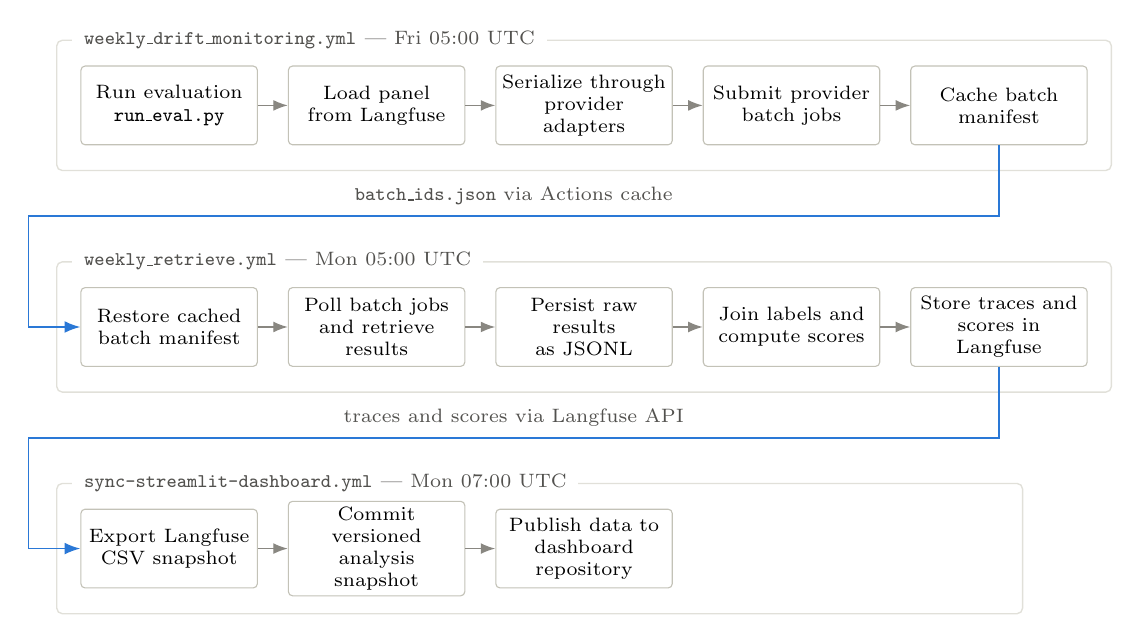
\begin{tikzpicture}[
  font=\scriptsize,
  >=Latex,
  wfstep/.style={
    draw=vizaxis, line width=0.4pt, rounded corners=1.5pt, fill=white,
    align=center, text width=21mm, minimum height=10mm, inner sep=2pt
  },
  lane/.style={draw=vizgrid, line width=0.5pt, rounded corners=2pt},
  lanelabel/.style={font=\scriptsize\bfseries, text=vizink, anchor=west, fill=white, inner xsep=1.5mm, inner ysep=0.4mm},
  flow/.style={->, vizmuted, line width=0.5pt},
  hand/.style={->, vizblue, line width=0.6pt},
  node distance=3.8mm,
]

% ---------------- lane 1: submit
\node[wfstep] (a1) {Run evaluation\\\texttt{run\_eval.py}};
\node[wfstep, right=of a1] (a2) {Load panel\\from Langfuse};
\node[wfstep, right=of a2] (a3) {Serialize through\\provider adapters};
\node[wfstep, right=of a3] (a4) {Submit provider\\batch jobs};
\node[wfstep, right=of a4] (a5) {Cache batch\\manifest};
\foreach \i/\j in {a1/a2, a2/a3, a3/a4, a4/a5} \draw[flow] (\i) -- (\j);

% ---------------- lane 2: retrieve
\node[wfstep, below=18mm of a1] (b1) {Restore cached\\batch manifest};
\node[wfstep, right=of b1] (b2) {Poll batch jobs\\and retrieve results};
\node[wfstep, right=of b2] (b3) {Persist raw results\\as JSONL};
\node[wfstep, right=of b3] (b4) {Join labels and\\compute scores};
\node[wfstep, right=of b4] (b5) {Store traces and\\scores in Langfuse};
\foreach \i/\j in {b1/b2, b2/b3, b3/b4, b4/b5} \draw[flow] (\i) -- (\j);

% ---------------- lane 3: dashboard
\node[wfstep, below=18mm of b1] (c1) {Export Langfuse\\CSV snapshot};
\node[wfstep, right=of c1] (c2) {Commit versioned\\analysis snapshot};
\node[wfstep, right=of c2] (c3) {Publish data to\\dashboard repository};
\foreach \i/\j in {c1/c2, c2/c3} \draw[flow] (\i) -- (\j);

% ---------------- lane frames and labels
\begin{scope}[on background layer]
  \node[lane, fit=(a1)(a5), inner xsep=3mm, inner ysep=3.2mm] (L1) {};
  \node[lane, fit=(b1)(b5), inner xsep=3mm, inner ysep=3.2mm] (L2) {};
  \node[lane, fit=(c1)(c3)(b5|-c1), inner xsep=3mm, inner ysep=3.2mm] (L3) {};
\end{scope}
\node[lanelabel] at ($(L1.north west)+(2mm,0)$)
  {\texttt{weekly\_drift\_monitoring.yml} \textnormal{--- Fri 05:00 UTC}};
\node[lanelabel] at ($(L2.north west)+(2mm,0)$)
  {\texttt{weekly\_retrieve.yml} \textnormal{--- Mon 05:00 UTC}};
\node[lanelabel] at ($(L3.north west)+(2mm,0)$)
  {\texttt{sync-streamlit-dashboard.yml} \textnormal{--- Mon 07:00 UTC}};

% ---------------- cross-lane handoffs, routed through the inter-lane gap
\coordinate (mid1) at ($(L1.south)!0.5!(L2.north)$);
\coordinate (mid2) at ($(L2.south)!0.5!(L3.north)$);

% routed left of the lane frames so they never cross a lane label
\coordinate (offL) at ($(L2.west)-(3.5mm,0)$);

\draw[hand] (a5.south) -- (a5.south|-mid1) -- (offL|-mid1) -- (offL|-b1) -- (b1.west);
\node[above=0.2mm, font=\scriptsize, text=vizink]
  at ($(a5.south|-mid1)!0.5!(offL|-mid1)$) {\texttt{batch\_ids.json} via Actions cache};

\draw[hand] (b5.south) -- (b5.south|-mid2) -- (offL|-mid2) -- (offL|-c1) -- (c1.west);
\node[above=0.2mm, font=\scriptsize, text=vizink]
  at ($(b5.south|-mid2)!0.5!(offL|-mid2)$) {traces and scores via Langfuse API};

\end{tikzpicture}

    \end{adjustbox}
    \caption{Scheduled GitHub Actions workflows. Each lane is one workflow; the two blue handoffs are the only state shared between them, which is what allows the asynchronous batch APIs to be polled in a later job.}
    \label{fig:ga-weekly-pipelines}
\end{figure}

\subsection{Workflow~1: Submit Batches}
\label{sec:batch-process}

Langfuse holds \(\mathcal{D}_N\) and the frozen \(\mathcal{D}_n\) with stable \texttt{custom\_id} join keys and the boolean label \texttt{campaign\_relevant} (Chapter~\ref{ch:data}). Weekly runs submit only \(\mathcal{D}_n\).

Rows normalize to \(\{\texttt{custom\_id},\;\texttt{body},\;\texttt{campaign\_relevant}\}\), with \texttt{body} built from \texttt{config/request\_template.json} plus the multimodal \texttt{input}. The same template is reused every week so temporal differences are not request-construction artefacts. Orchestrator \texttt{run\_eval.py} loads the panel, ensures Gemini image uploads when needed, and dispatches each model to \texttt{batch\_*.py}. Adapters serialize to the provider batch format, upload JSONL, submit the job, and write the run manifest \texttt{data/batch\_ids.json} (\texttt{run\_id}, \texttt{subset\_size}, per-model batch IDs) into the Actions cache for retrieval.

The prediction task is identical across providers: JSON boolean \texttt{campaign\_relevant} under a schema-constrained output. Adapter differences are only transport-level (Table~\ref{tab:provider-adapters}). Claude sanitizes \texttt{custom\_id} on the wire and remaps on download. Gemini replaces image URLs with Files API URIs via \texttt{upload\_gemini\_images.py} and \texttt{data/gemini\_image\_cache.json} (TTL \(\approx\) 47~h). Across providers the output schema is \(\{\texttt{campaign\_relevant},\; \texttt{relevancy\_reasoning}\}\).

\begin{table}[htbp]
\centering
\footnotesize
\caption{Adapter-layer mapping for one shared task and one shared request body: what changes per provider and why.}
\label{tab:provider-adapters}
\setlength{\tabcolsep}{5pt}
\renewcommand{\arraystretch}{1.25}
\begin{tabular}{|p{2.0cm}|p{4.2cm}|p{8.1cm}|}
\hline
Provider & Schema / response constraint & Provider-specific preprocessing \\
\hline
OpenAI & \texttt{text.format} with JSON schema & Reuse canonical multimodal \texttt{input}; keep image URLs as-is \\
\hline
Gemini & \texttt{responseSchema} with JSON MIME type & Convert URLs to Files API \texttt{fileUri}; use upload cache (TTL \(\approx\) 47 h); skip rows with missing media \\
\hline
Claude & Anthropic \texttt{output\_config} schema & Sanitize \texttt{custom\_id} for submission; remap IDs on result download \\
\hline
\end{tabular}
\end{table}

\textbf{Output.} The submission workflow produces \texttt{data/batch\_ids.json} and the submitted JSONL files under \texttt{batches/}.

\subsection{Workflow~2: Retrieve and Ingest}
\label{sec:metrics-dashboard}

\texttt{poll\_and\_ingest.py} restores the manifest, polls until completion, and downloads JSONL into \texttt{data/results/}. Then \texttt{ingest.py} normalizes each response, joins \texttt{campaign\_relevant} to ground truth via \texttt{custom\_id}, maps token usage to \texttt{cost\_usd} via \texttt{config/models.yaml}, and writes Langfuse traces with scores.

Table~\ref{tab:batch-pricing-examples} lists batch prices for the monitored roster; \texttt{models.yaml} also carries unused candidates for future adds.

\begin{table}[htbp]
    \centering
    \caption{Batch-API prices per one million tokens (USD) for the monitored models, as of 16~March~2026. Claude batch prices are half the corresponding standard prices.}
    \label{tab:batch-pricing-examples}
    \begin{tabular}{lrr}
        \toprule
        Model & Input & Output \\
        \midrule
        \texttt{gpt-5.4-2026-03-05}      & 1.25  & 7.50  \\
        \texttt{gpt-5.2}                 & 0.875 & 7.00  \\
        \texttt{gpt-5.1}                 & 0.625 & 5.00  \\
        \texttt{gpt-5}                   & 0.625 & 5.00  \\
        \texttt{gpt-5-mini}              & 0.125 & 1.00  \\
        \texttt{gpt-5-nano}              & 0.025 & 0.20  \\
        \texttt{gpt-4.1-mini}            & 0.20  & 0.80  \\
        \texttt{gpt-4.1-nano}            & 0.05  & 0.20  \\
        \midrule
        \texttt{gemini-2.5-flash}        & 0.15  & 1.25  \\
        \midrule
        \texttt{claude-sonnet-4-6}       & 1.78 & 8.92  \\
        \texttt{claude-sonnet-4-5}       & 1.78 & 8.92  \\
        \texttt{claude-haiku-4-5}        & 0.59 & 2.97  \\
        \bottomrule
    \end{tabular}
\end{table}

Trace scores used later: \texttt{accuracy} (\(1/0\) match), \texttt{error\_type} (TP/FP/TN/FN), and \texttt{cost\_usd}. Precision, recall, and F1 follow Section~\ref{sec:classification-metrics}.

\subsection{Workflow~3: Dashboard Sync}

\texttt{sync-streamlit-dashboard.yml} exports traces/scores via \texttt{export\_langfuse\_csv.py} into committed CSVs in \texttt{gocomo/llm-batch-eval}, then mirrors \texttt{streamlit\_app/} to \texttt{GeorgiiBurdinComo/llm-eval-dashboard}. Tabs: Overview (accuracy/cost over time), McNemar (contingency tables and exact \(p\)), Utility (\(E_t[\mathcal{C}](m)\) with \(R=C_{\mathrm{FP}}/C_{\mathrm{FN}}\)).

\subsection{Artifacts and Cross-Step Data Flow}
\label{sec:artifacts-data-flow}

Workflows share only files: \texttt{data/batch\_ids.json}, \texttt{batches/}, \texttt{data/results/}, Langfuse, then CSV snapshots. Any stage can be replayed from the previous artifact without repeating provider calls.

\FloatBarrier

\section{Experimental Setup}
\label{sec:experimental-design}

Datasets and roster are those of Chapter~\ref{ch:data} and Table~\ref{tab:monitored-models}. This chapter reports the frozen-panel baseline, longitudinal McNemar evidence, and the corrective-action comparison panel. Figure~\ref{fig:run-decision-logic} is the operational loop; prompt optimisation is shown as a branch but only monitoring and comparison are evaluated here. The realized degradation episode is Chapter~\ref{chap:degradation-case-study}.

\FloatBarrier
\begin{figure}[H]
    \centering
    \begin{adjustbox}{max width=0.92\textwidth}
    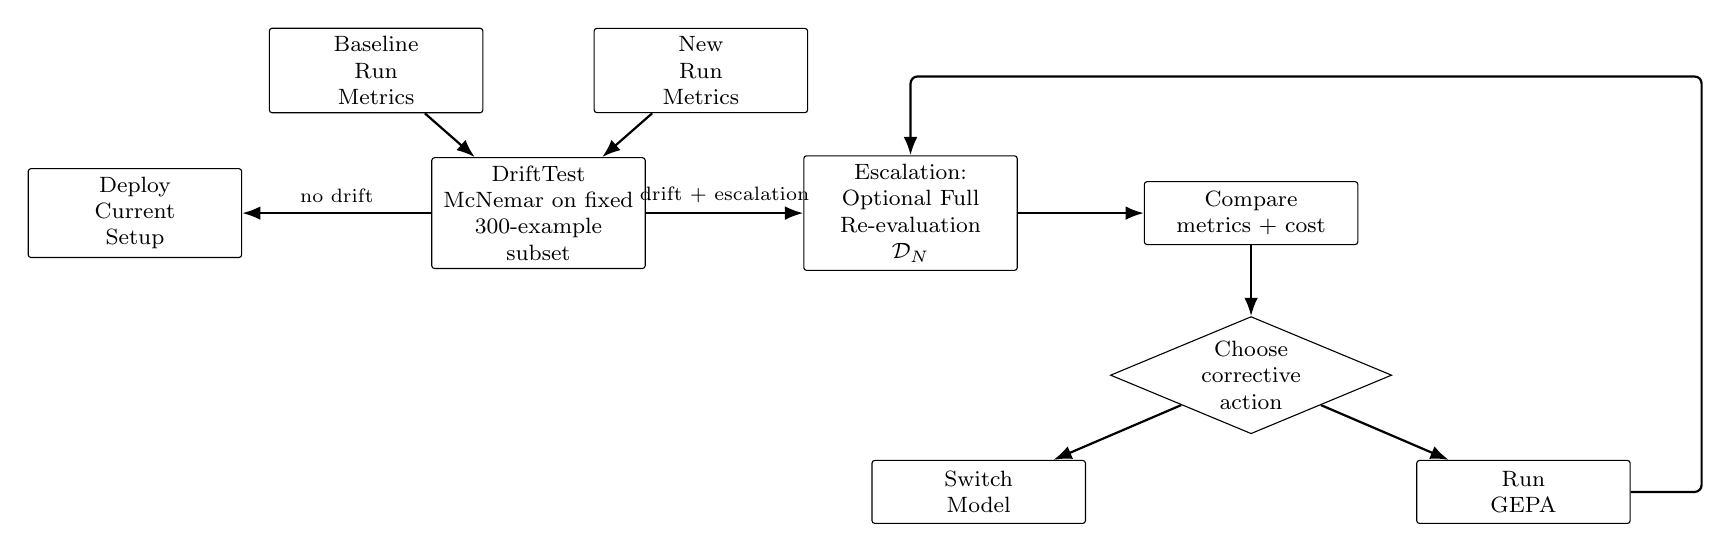
\begin{tikzpicture}[
    >=Latex,
    node distance=9mm and 14mm
    ]
    
    \node[figbox] (baseline) {Baseline\\Run\\Metrics};
    \node[figbox, right=of baseline] (newrun) {New\\Run\\Metrics};
    
    \node[figbox, below=11mm of $(baseline)!0.5!(newrun)$] (drift) {DriftTest\\McNemar on fixed\\300-example subset};
    
    \node[figbox, left=24mm of drift] (deploy) {Deploy\\Current\\Setup};
    \node[figbox, right=20mm of drift] (reeval) {Escalation:\\Optional Full\\Re-evaluation\\$ \mathcal{D}_N $};
    \node[figbox, right=16mm of reeval] (metriccost) {Compare\\metrics + cost};
    
    \node[figdiamond, below=9mm of metriccost] (decision) {Choose\\corrective\\action};
    
    \node[figbox, below left=7mm and 12mm of decision] (switch) {Switch\\Model};
    \node[figbox, below right=7mm and 12mm of decision] (gepa) {Run\\GEPA};
    
    \draw[figarrow] (baseline) -- (drift);
    \draw[figarrow] (newrun) -- (drift);
    
    \draw[figarrow] (drift) -- node[midway, above, font=\scriptsize]{no drift} (deploy);
    \draw[figarrow] (drift) -- node[midway, above, font=\scriptsize]{drift + escalation} (reeval);
    
    \draw[figarrow] (reeval) -- (metriccost);
    \draw[figarrow] (metriccost) -- (decision);
    
    \draw[figarrow] (decision) -- (switch);
    \draw[figarrow] (decision) -- (gepa);
    
    \coordinate (loopabove) at ($(reeval.north)+(0,1.0)$);
    \draw[figarrow, rounded corners=2.5pt]
      (gepa.east) -- ++(0.9,0) |- (loopabove) -- (reeval.north);
    
    \end{tikzpicture}
    \end{adjustbox}
    \caption{Decision logic after a monitoring run: McNemar drift on the fixed \(n=300\) panel, optional full-benchmark re-evaluation on \(\mathcal{D}_N\), then metric/cost comparison and corrective action (model switch or GEPA loop).}
    \label{fig:run-decision-logic}
\end{figure}
\FloatBarrier

\section{Results}

\subsection{Baseline and Instantiated Monitoring Subset}
\label{sec:baseline-subset}

A one-time \(\mathcal{D}_N\) run seeds the disagreement construction of Chapter~\ref{ch:data}; the resulting \(n=300\) panel is frozen in Langfuse. Table~\ref{tab:phase1-baseline-snapshot} is a descriptive baseline excerpt on \(\mathcal{D}_n\) (metrics export, last score day 2026-04-13).

\begin{table}[htbp]
    \centering
    \caption{Baseline excerpt: classification metrics on the frozen monitoring subset (metrics export, last score day 2026-04-13).}
    \label{tab:phase1-baseline-snapshot}
    \begin{tabular}{lccccc}
        \toprule
        Model & $n$ & Accuracy & Precision & Recall & F1 \\
        \midrule
        \texttt{gpt-4.1-mini} & 300 & 0.8033 & 0.9948 & 0.7680 & 0.8668 \\
        \texttt{gpt-4.1-nano} & 300 & 0.7000 & 0.9444 & 0.6800 & 0.7907 \\
        \bottomrule
    \end{tabular}
\end{table}

The baseline fixes the initial error profile against which later runs are compared; fallback choice depends on which error type is costly under Chapter~\ref{ch:cost-deployment-utility}.

\subsection{Realized discordance}
\label{sec:realized-discordance}

The panel size in Section~\ref{sec:monitoring-sample-size} was derived from a pilot discordance rate of $\hat\rho=0.114$, measured by running $\mathcal{D}_N$ twice two days apart. Table~\ref{tab:discordance} reports the discordance actually observed between each model's baseline run and its later runs.

\begin{table}[htbp]
    \centering
    \footnotesize
    \caption{Discordance rate $(b+c)/n$ between each model's onset baseline and later
    scheduled panel runs. Pooled median 0.027.}
    \label{tab:discordance}
    \begin{tabular}{lcccc}
    \toprule
    Model & Comparisons & Median & Min & Max \\
    \midrule
    \texttt{gpt-4.1-nano} & 16 & 0.152 & 0.124 & 0.187 \\
    \texttt{gpt-5-nano} & 15 & 0.124 & 0.094 & 0.149 \\
    \texttt{gpt-5-mini} & 15 & 0.080 & 0.070 & 0.104 \\
    \texttt{gpt-4.1-mini} & 16 & 0.062 & 0.040 & 0.206 \\
    \texttt{claude-haiku-4-5} & 14 & 0.034 & 0.015 & 0.049 \\
    \texttt{claude-sonnet-4-5} & 14 & 0.030 & 0.023 & 0.053 \\
    \texttt{gpt-5.1} & 15 & 0.020 & 0.010 & 0.034 \\
    \texttt{gemini-2.5-flash} & 12 & 0.017 & 0.010 & 0.023 \\
    \texttt{claude-sonnet-4-6} & 14 & 0.015 & 0.008 & 0.023 \\
    \texttt{gpt-5.4} & 13 & 0.013 & 0.007 & 0.017 \\
    \texttt{gpt-5.2} & 14 & 0.010 & 0.003 & 0.013 \\
    \texttt{gpt-5} & 15 & 0.007 & 0.003 & 0.010 \\
    \bottomrule
    \end{tabular}
\end{table}


The pooled median is $0.033$, well below the pilot value. Two things drive the gap. First, the pilot measured one model; the roster spans a wide stability range, from \texttt{gpt-4.1-nano} at $0.156$ down to \texttt{gpt-5} at $0.007$. Second, the pilot model was the production model of the time, which sat in the churn-heavy part of that range.

The consequence is a power loss concentrated in the stable models. The planning equation~\eqref{eq:planning-discordant-m} needs $m\approx 31$ discordant pairs to detect $\delta=0.05$ at $80\%$ power. At $\rho=0.007$, a 300-item panel yields $m\approx 2$. For \texttt{gpt-5} and \texttt{gpt-5.2} the panel is therefore too small to detect a five-point drop, and their flat monitoring series should be read as uninformative rather than as evidence of stability. For the models at $\rho\ge 0.10$ the panel delivers $m\approx 30$ or more and the sizing assumption holds.

The panel was sized once, for one model, and then frozen. Per-model sizing --- a larger panel for low-churn models --- would fix this, at proportionally higher cost per run.

\subsection{Longitudinal Monitoring Results}
\label{sec:drift-results}

This subsection checks whether repeated evaluation on the fixed monitoring subset shows meaningful temporal changes in model behaviour. Since the panel is fixed, changes in the paired discordance counts \((b,c)\) reflect changed predictions rather than a changed sample.

\begin{table}[htbp]
    \centering
    \caption{McNemar table for \texttt{gpt-4.1-mini} between 6~April~2026 and 13~April~2026 on \(\mathcal{D}_n\) ($n=299$).}
    \label{tab:mcnemar_gpt41mini}
    \begin{tabular}{lcc}
        \toprule
        & 2026-04-13 correct & 2026-04-13 wrong \\
        \midrule
        2026-04-06 correct & 230 & 10 \\
        2026-04-06 wrong   & 10  & 49 \\
        \bottomrule
    \end{tabular}
\end{table}

\begin{table}[htbp]
    \centering
    \caption{McNemar table for \texttt{gpt-4.1-nano} between 6~April~2026 and 13~April~2026 on \(\mathcal{D}_n\).}
    \label{tab:mcnemar_gpt41nano}
    \begin{tabular}{lcc}
        \toprule
        & 2026-04-13 correct & 2026-04-13 wrong \\
        \midrule
        2026-04-06 correct & 184 & 22 \\
        2026-04-06 wrong   & 26  & 68 \\
        \bottomrule
    \end{tabular}
\end{table}

Two recent run pairs show the range of outcomes. For \texttt{gpt-4.1-mini}, the comparison from 6~April~2026 to 13~April~2026 gives the contingency table in Table~\ref{tab:mcnemar_gpt41mini}. The discordant counts are \((b,c)=(10,10)\), so gains and losses balance exactly and there is no directional change.

For \texttt{gpt-4.1-nano}, the corresponding comparison in Table~\ref{tab:mcnemar_gpt41nano} gives \((b,c)=(22,26)\): 48 instances change status, with 22 regressions and 26 recoveries. The one-sided McNemar test does not reach \(\alpha=0.05\). Thus, despite noticeable churn, the net direction is not degradation under the alert rule from Chapter~\ref{ch:drift}.

These two examples show two different situations on the fixed panel: balanced movement with no directional evidence (\texttt{gpt-4.1-mini}) and high-churn but non-degrading movement (\texttt{gpt-4.1-nano}). In both cases, the correct operational response is continued monitoring together with preparation of fallback comparisons on the metric and cost panel.

\subsection{Alert counts over the full monitoring period}
\label{sec:method-comparison}

The monitoring series covers 8~March to 27~July~2026 and yields 265 baseline-to-current comparisons over 19 models. Twelve model-days are full-benchmark runs of about $1{,}190$ items rather than panel runs; these are escalation and prompt-transfer evaluations, not part of the weekly loop, and they are excluded from the drift series. Mixing them in would compare a panel run against a benchmark run and attribute the difference to the model.

\begin{table}[htbp]
    \centering
    \caption{Alert counts over 173 baseline-to-later comparisons
    (12 models, scheduled panel runs, 15~March--6~July~2026).
    Holm correction is applied once to the full primary family.}
    \label{tab:alert-counts}
    \begin{tabular}{lr}
    \toprule
    Rule & Alerts \\
    \midrule
    $b>c$, $p_{\mathrm{exact}}<0.05$ (uncorrected) & 3 \\
    $b>c$, Holm-adjusted $p<0.05$ & 1 \\
    Holm and $\Delta A_{\mathrm{paired}}\le-3$pp (operational) & 1 \\
    \midrule
    $\Delta A_{\mathrm{paired}}\le-3$pp alone & 2 \\
    $\Delta A_{\mathrm{paired}}\le-5$pp alone & 1 \\
    \bottomrule
    \end{tabular}
\end{table}


Table~\ref{tab:alert-counts} gives the alert counts. At the nominal $\alpha=0.05$ the rule fires 13 times. The Bonferroni correction of~\eqref{eq:bonferroni} reduces this to 3. Adding a three-point relevance floor removes nothing further: all three surviving comparisons are drops of $4.7$pp or more, so on this data the floor is inert and the correction is doing the filtering.

The three surviving comparisons are not three episodes. Two of them are \texttt{gpt-4.1-mini} against its 8~March baseline on 22 and 23~March, which is one event observed on two consecutive days; Chapter~\ref{chap:degradation-case-study} treats it in full. The third is \texttt{gpt-5-mini} on 6~April, at $-4.7$pp with $p=1.3\times10^{-3}$, and it needs a different reading.

\paragraph{The \texttt{gpt-5-mini} alert is baseline noise.}
\texttt{gpt-5-mini} scores $0.940$ on the 8~March baseline and then sits between $0.893$ and $0.933$ for the following twenty-two runs, with no trend. The baseline is the highest single value in the series. Every later comparison therefore inherits a small negative offset, and nine of the twenty-two clear $p<0.05$ before correction. The 6~April run is simply the lowest of them. Reading this as a provider-side change would be wrong: nothing steps, and the post-baseline level is flat.

This is the cost of the fixed-baseline design noted in Section~\ref{sec:baseline-multiplicity}. Anchoring on one batch makes the entire series inherit that batch's sampling error, and a baseline that happens to land high manufactures a persistent apparent decline. Bonferroni suppresses eight of the nine, but not the largest, so multiplicity control alone does not remove the problem. Two mitigations are available and neither was in place here: pool the first two runs into the baseline, or require an alert to repeat before it is acted on. On this data the second rule would have retained the \texttt{gpt-4.1-mini} event, which fired on two consecutive days, and dropped the \texttt{gpt-5-mini} alert, which fired once.

By simple thresholds, a $-3$pp rule fires 15 times and a $-5$pp rule twice. The $-5$pp rule selects exactly the two \texttt{gpt-4.1-mini} comparisons --- on this data the crudest rule available recovers the one real event and nothing else. The paired test earns its place not through a lower alert count but by reporting $b$ and $c$ separately, which is what makes the \texttt{gpt-5-mini} case diagnosable at all: a threshold rule reports only that accuracy is down.

\subsection{Candidate Comparison for Corrective Action}
\label{sec:cost-aware-comparison}

After escalation, candidates are compared on accuracy, precision, recall, F1, and mean cost. Table~\ref{tab:model-metrics-snapshot} is the \(\mathcal{D}_n\) profile (confusion counts plus derived metrics; \texttt{cost\_usd} from Section~\ref{sec:metrics-dashboard}). Final expected-cost ranking uses \(\mathcal{D}_N\) under Chapter~\ref{ch:cost-deployment-utility} (Section~\ref{sec:selection-bias}).

\begin{table}[htbp]
    \centering
    \footnotesize
    \caption{Exported snapshot of confusion counts and classification metrics per candidate (evaluation on \(\mathcal{D}_n\)).}
    \label{tab:model-metrics-snapshot}
    \begin{adjustbox}{max width=\linewidth}
    % Auto-generated — last score day 2026-03-28
% % Auto-generated — last score day 2026-03-28
% \input{metrics_tabular.tex} inside your table environment
\begin{tabular}{lrrrrrrrrrrrr}
\toprule
model & n & tp & fp & tn & fn & accuracy & precision & recall & f1 & specificity & balanced\_accuracy & pr\_auc \\
\midrule
gpt-4.1-mini & 299 & 190 & 1 & 49 & 59 & 0.7993 & 0.9948 & 0.7631 & 0.8636 & 0.9800 & 0.8715 & 0.9776 \\
gpt-4.1-nano & 300 & 178 & 8 & 42 & 72 & 0.7333 & 0.9570 & 0.7120 & 0.8165 & 0.8400 & 0.7760 & 0.9545 \\
\bottomrule
\end{tabular}

 inside your table environment
\begin{tabular}{lrrrrrrrrrrrr}
\toprule
model & n & tp & fp & tn & fn & accuracy & precision & recall & f1 & specificity & balanced\_accuracy & pr\_auc \\
\midrule
gpt-4.1-mini & 299 & 190 & 1 & 49 & 59 & 0.7993 & 0.9948 & 0.7631 & 0.8636 & 0.9800 & 0.8715 & 0.9776 \\
gpt-4.1-nano & 300 & 178 & 8 & 42 & 72 & 0.7333 & 0.9570 & 0.7120 & 0.8165 & 0.8400 & 0.7760 & 0.9545 \\
\bottomrule
\end{tabular}


    \end{adjustbox}
\end{table}

Read confusion counts first, then derived metrics, then \(E_t[\mathcal{C}]\) on \(\mathcal{D}_N\). Similar accuracy can hide very different FP/FN mixes; which model wins depends on campaign costs via \(R=C_{\mathrm{FP}}/C_{\mathrm{FN}}\).
\section{Limitations}
\label{sec:error-analysis}

\begin{itemize}
    \item Provider state is unobserved; drift is inferred only from output changes on the fixed panel.
    \item Cost depends on provider pricing and tokenization, so monetary comparisons may change even when the confusion structure stays the same.
    \item Every comparison reuses one baseline run, so sampling error in that run propagates to the whole series for that model (Section~\ref{sec:method-comparison}).
    \item The panel was sized from a single pilot discordance estimate. For the most stable models the realized discordance leaves the panel underpowered at the design effect size (Section~\ref{sec:realized-discordance}).
\end{itemize}

The degradation episode itself is Chapter~\ref{chap:degradation-case-study}.


\chapter{Experimental Results}
\label{chap:experimental-results}

This chapter reports the recorded monitoring window from 15~March to 6~July~2026 for the 12 recurring monitoring series and the later common-case deployment comparison for the eight candidate models with shared full-benchmark outputs on 22~May~2026.

\section{Monitoring results}
\label{sec:drift-results}

The timeline contains 187 eligible runs. The recurring monitored series are \texttt{claude-haiku-4-5}, \texttt{claude-sonnet-4-5}, \texttt{claude-sonnet-4-6}, \texttt{gemini-2.5-flash}, \texttt{gpt-4.1-mini}, \texttt{gpt-4.1-nano}, \texttt{gpt-5}, \texttt{gpt-5-mini}, \texttt{gpt-5-nano}, \texttt{gpt-5.1}, \texttt{gpt-5.2}, and \texttt{gpt-5.4}. For each recurring model, the first recorded run was a full-benchmark baseline on \(\mathcal{D}_N\); later routine monitoring runs used the frozen \(n=300\) panel, and paired monitoring comparisons restricted both runs to the common panel items. These twelve recurring model labels therefore contribute 185 runs and 173 baseline-to-later paired comparisons. Missing outputs are removed pairwise, so the effective sample size can be below 300.

The two singleton labels are \texttt{gemini-2.0-flash} and \texttt{gpt-5.4-2026-03-05}; each appears once. A model's first recorded run is its full-benchmark baseline, so these two runs remain recorded baselines until a later comparison exists. The frozen labelled sets make this straightforward:
\begin{enumerate}
    \item a newly released model is scored on the same posts as the existing candidates;
    \item its first run is compared with the other series from the same period;
    \item later runs are paired against that model's own first-run baseline.
\end{enumerate}

At the one-sided nominal level \(\alpha=.05\), three comparisons produced monitoring signals with \(p_{\mathrm{exact}}<.05\). These signals opened review on the fixed panel; deployment significance was determined separately.

\begin{table}[htbp]
    \centering
    \small
    \caption{Canonical monitoring summary, 15~March--6~July~2026.}
    \label{tab:canonical-monitoring-summary}
    % Generated from canonical_summary.json; do not edit.
\begin{tabular}{lr}
\toprule
Quantity & Value \\
\midrule
Eligible scheduled runs & 187 \\
Models with comparisons & 12 \\
Baseline-to-later comparisons & 173 \\
Nominal one-sided \(p<0.05\) & 3 \\
\bottomrule
\end{tabular}

\end{table}
\provline{P4}

\begin{figure}[htbp]
    \centering
    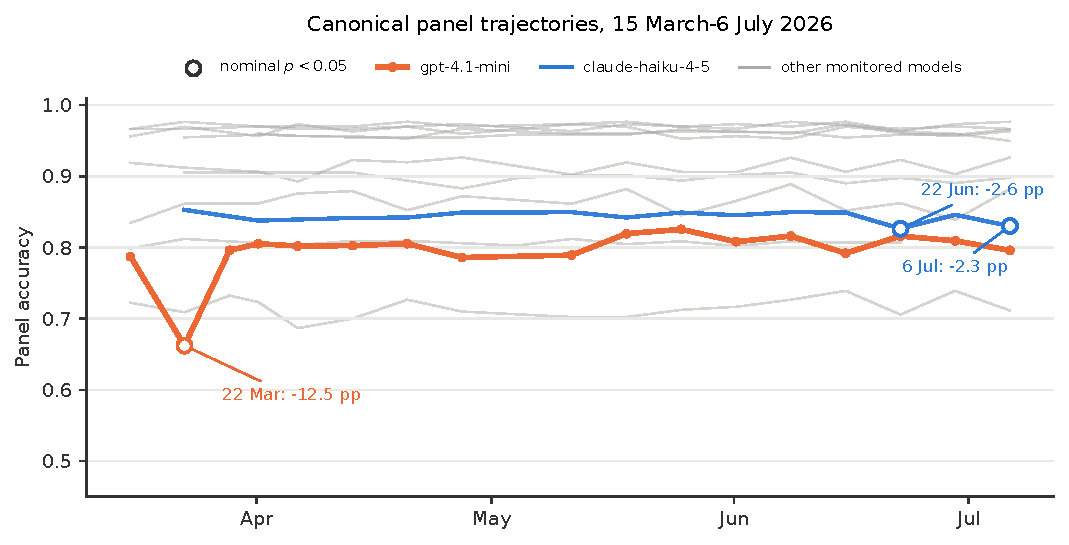
\includegraphics[width=\linewidth]{assets/evidence/fig_canonical_monitoring_trajectory.pdf}
    \caption[Canonical panel-accuracy trajectories]{Panel accuracy for the 12 recurring monitoring series. Open markers show the three nominal one-sided \(p_{\mathrm{exact}}<.05\) signals. The orange and blue trajectories identify the two models that produced them; grey series provide same-period context.}
    \label{fig:canonical-monitoring-trajectory}
\end{figure}
\FloatBarrier

Table~\ref{tab:nominal-mcnemar} reports the paired correctness counts for the three comparisons with nominal one-sided signals. McNemar's test uses the discordant cells: \(b\) counts items that changed from correct to wrong, and \(c\) counts items that changed from wrong to correct. The three comparisons are:
\begin{enumerate}
    \item \texttt{gpt-4.1-mini}, 15~March--22~March: \(b=49\), \(c=12\), \(n=296\);
    \item \texttt{claude-haiku-4-5}, 22~March--22~June: \(b=9\), \(c=2\), \(n=265\);
    \item \texttt{claude-haiku-4-5}, 22~March--6~July: \(b=7\), \(c=1\), \(n=265\).
\end{enumerate}

None of these two models were deployed in production, so no production deployment change was made.
\begin{table}[htbp]
    \centering
    \small
    \caption[Nominal McNemar tables]{Paired correctness counts for the three comparisons with one-sided \(p_{\mathrm{exact}}<.05\).}
    \label{tab:nominal-mcnemar}
    % Generated from baseline_to_later_mcnemar.csv; do not edit.
\begin{minipage}[t]{0.32\linewidth}
\centering
\texttt{gpt-4.1-mini}\\
{\scriptsize 15~Mar--22~Mar, \(n=296\)}\\[3pt]
\begin{tabular}{c|cc}
 & later \(+\) & later \(-\) \\
\hline
base \(+\) & 184 & \(b=49\) \\
base \(-\) & \(c=12\) & 51 \\
\end{tabular}\\[3pt]
{\scriptsize \(\Delta=-12.5\)\,pp, \(p_{\mathrm{exact}}=9.849\times10^{-7}\)}
\end{minipage}
\hfill
\begin{minipage}[t]{0.32\linewidth}
\centering
\texttt{claude-haiku-4-5}\\
{\scriptsize 22~Mar--22~Jun, \(n=265\)}\\[3pt]
\begin{tabular}{c|cc}
 & later \(+\) & later \(-\) \\
\hline
base \(+\) & 217 & \(b=9\) \\
base \(-\) & \(c=2\) & 37 \\
\end{tabular}\\[3pt]
{\scriptsize \(\Delta=-2.64\)\,pp, \(p_{\mathrm{exact}}=0.0327\)}
\end{minipage}
\hfill
\begin{minipage}[t]{0.32\linewidth}
\centering
\texttt{claude-haiku-4-5}\\
{\scriptsize 22~Mar--6~Jul, \(n=265\)}\\[3pt]
\begin{tabular}{c|cc}
 & later \(+\) & later \(-\) \\
\hline
base \(+\) & 219 & \(b=7\) \\
base \(-\) & \(c=1\) & 38 \\
\end{tabular}\\[3pt]
{\scriptsize \(\Delta=-2.26\)\,pp, \(p_{\mathrm{exact}}=0.0352\)}
\end{minipage}

\end{table}
\provline{P4}
\FloatBarrier

\paragraph{The March signal and rebound.}
For \texttt{gpt-4.1-mini}, the 15--22~March comparison in Table~\ref{tab:nominal-mcnemar} produced the strongest signal. Panel accuracy fell from \(0.7872\) to \(0.6622\), a change of \(-12.5\) percentage points, and the one-sided exact p-value was \(9.849\times10^{-7}\).

The next run, 22--28~March, reversed the movement: on 297 complete pairs accuracy rose from \(0.6633\) to \(0.7946\), with 11 regressions and 50 improvements. From 15 to 28~March the net change was \(+0.67\) percentage points, so the episode did not persist. \texttt{gpt-4.1-mini} was only a monitored candidate, therefore no production deployment change.

No model-specific incident or update notice for \texttt{gpt-4.1-mini} was listed in the public OpenAI status history for 15 or 22~March~2026~\cite{openai2026status}. The episode therefore illustrates the intended role of the monitor: it surfaced an unexplained provider-side behaviour change on the fixed panel without any contemporaneous public notice for that model was available.
\provref{P4}

\begin{figure}[htbp]
    \centering
    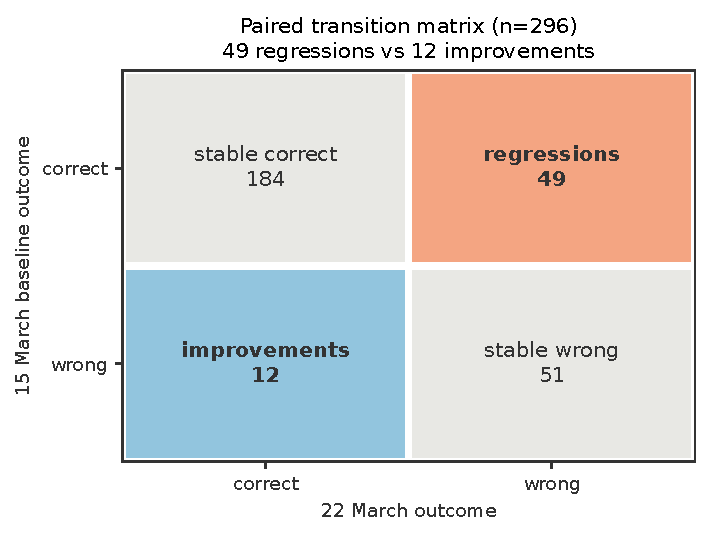
\includegraphics[width=0.68\linewidth]{assets/evidence/fig_canonical_mcnemar_matrix.pdf}
    \caption[Paired transitions behind the March signal]{Paired correctness transitions for \texttt{gpt-4.1-mini}, 15--22~March. McNemar's test ignores the two grey concordant cells and evaluates the imbalance between 49 regressions and 12 improvements.}
    \label{fig:canonical-mcnemar-matrix}
\end{figure}
\FloatBarrier

\section{Monitoring cost}
\label{sec:monitoring-cost}

\begin{table}[htbp]
    \centering
    \small
    \caption[Observed panel and benchmark API costs]{Observed API cost per evaluation sweep. The production set is \texttt{gpt-5-mini}, \texttt{gpt-5-nano}, and \texttt{gpt-5}.}
    \label{tab:monitoring-cost}
    % Generated from assets/drift/monitoring_cost.json; do not edit.
\begin{tabular}{lrr}
\toprule
Evaluation scope & Eight models & Three production models \\
\midrule
Full benchmark & \$43.10 & \$9.53 \\
Sentinel panel & \$12.26 & \$2.74 \\
\bottomrule
\end{tabular}

\end{table}

That paired sensitivity is inexpensive enough to run routinely. For the three production models---\texttt{gpt-5-mini}, \texttt{gpt-5-nano}, and \texttt{gpt-5}---one panel sweep cost \(\$2.74\), compared with \(\$9.53\) for a full-benchmark sweep. Weekly panel monitoring therefore costs approximately \(\$142.42\) per year in API charges.

The error cost of an undetected episode can be estimated conditionally on the penalties used in Section~\ref{sec:cost-aware-comparison}. On the 296 items shared by the \texttt{gpt-4.1-mini} baseline and signal runs, the confusion counts changed from \((\mathrm{FP},\mathrm{FN})=(2,61)\) to \((0,100)\). Holding inference price fixed, the resulting incremental error loss per affected classification is
\[
    \Delta L_{\mathrm{err}}
    =\frac{0.155(0-2)+0.031(100-61)}{296}
    =\$0.003037.
\]

\begin{table}[htbp]
    \centering
    \small
    \caption[Production-model monitoring scenarios]{Model-specific monitoring costs and break-even volumes under the observed episode's incremental error loss of \(\$0.003037\) per affected classification. Costs are USD; annual panel cost is \(52\times\) weekly panel cost, and weekly break-even volume is \(\text{panel cost}/0.003037=\text{annual panel cost}/(52\times0.003037)\).}
    \label{tab:production-monitoring-scenarios}
    % Generated from assets/drift/monitoring_cost.json; do not edit.
\begin{tabular}{lrrrr}
\toprule
Model & Panel & Full & Annual panel & Weekly break-even \\
\midrule
\texttt{gpt-5-mini} & \$0.43 & \$1.54 & \$22.37 & 142 posts \\
\texttt{gpt-5-nano} & \$0.11 & \$0.39 & \$5.79 & 37 posts \\
\texttt{gpt-5} & \$2.20 & \$7.60 & \$114.26 & 723 posts \\
\bottomrule
\end{tabular}

\end{table}
\provline{P5}

For the three production models, weekly panel cost ranges from \(\$0.11\) to \(\$2.20\), and the corresponding break-even volume ranges from 37 to 723 affected classifications under this scenario. Other failure patterns imply different thresholds. This supports the operational case for running the fixed panel routinely as a review trigger; model replacement still depends on the separate full-benchmark comparison in Section~\ref{sec:cost-aware-comparison}.

\section{Cost-aware comparison}
\label{sec:cost-aware-comparison}

The deployment comparison uses the 22~May common complete-case intersection for the eight candidate models with shared full-benchmark outputs on that date: 1113 items observed for all eight models. This avoids changing the evaluated item set across candidates. The illustrative operating point is
\[
    w=\frac{C_{\mathrm{FN}}}{C_{\mathrm{FP}}}=0.2,
    \qquad
    \lambda=C_{\mathrm{FP}}+C_{\mathrm{FN}}=0.186,
\]
which is equivalent to \(C_{\mathrm{FP}}=0.155\) and \(C_{\mathrm{FN}}=0.031\) USD, in addition to mean inference cost. At this operating point, a false positive is assigned five times the cost of a false negative. This reflects the operational burden of sending irrelevant posts into downstream processing.

\begin{table}[htbp]
    \centering
    \small
    \caption{Complete-case results on 22~May 2026 (\(n_t=1113\)); \(w=0.2\), \(\lambda=0.186\).}
    \label{tab:canonical-cost-comparison}
    % Generated from deployment_cost_may22.csv; do not edit.
\begin{tabular}{lrrrrrrr}
\toprule
Model & Accuracy & Precision & Recall & $c_t(m)$ (USD) & FP & FN & Loss \\
\midrule
\texttt{gpt-5-mini} & 0.940 & 0.991 & 0.901 & 0.0013 & 5 & 62 & 0.0037 \\
\texttt{gpt-5-nano} & 0.901 & 0.992 & 0.834 & 0.0003 & 5 & 105 & 0.0039 \\
\texttt{gpt-5.1} & 0.972 & 0.973 & 0.976 & 0.0053 & 16 & 15 & 0.0080 \\
\texttt{gpt-5} & 0.978 & 0.966 & 0.995 & 0.0065 & 21 & 3 & 0.0095 \\
\texttt{gpt-4.1-mini} & 0.754 & 0.994 & 0.572 & 0.0019 & 2 & 271 & 0.0097 \\
\texttt{gpt-5.2} & 0.979 & 0.973 & 0.989 & 0.0084 & 16 & 7 & 0.0108 \\
\texttt{gpt-4.1-nano} & 0.778 & 0.897 & 0.681 & 0.0007 & 49 & 198 & 0.0130 \\
\texttt{gpt-5.4} & 0.970 & 0.970 & 0.976 & 0.0115 & 18 & 15 & 0.0144 \\
\bottomrule
\end{tabular}

\end{table}
\provline{P5}

\texttt{gpt-5-mini} minimises plug-in loss at \(0.003698\). It balances low inference cost with five false positives and 62 false negatives. The cheaper \texttt{gpt-5-nano} is a close second at \(0.003950\): its lower inference cost does not offset 105 false negatives. The accuracy leader \texttt{gpt-5.2} reaches \(0.97932\) accuracy but has loss \(0.010835\), mainly because its inference cost and 16 false positives are expensive under the stated business asymmetry. Therefore neither maximum accuracy nor minimum API price alone selects the preferred deployment model.

\begin{figure}[htbp]
    \centering
    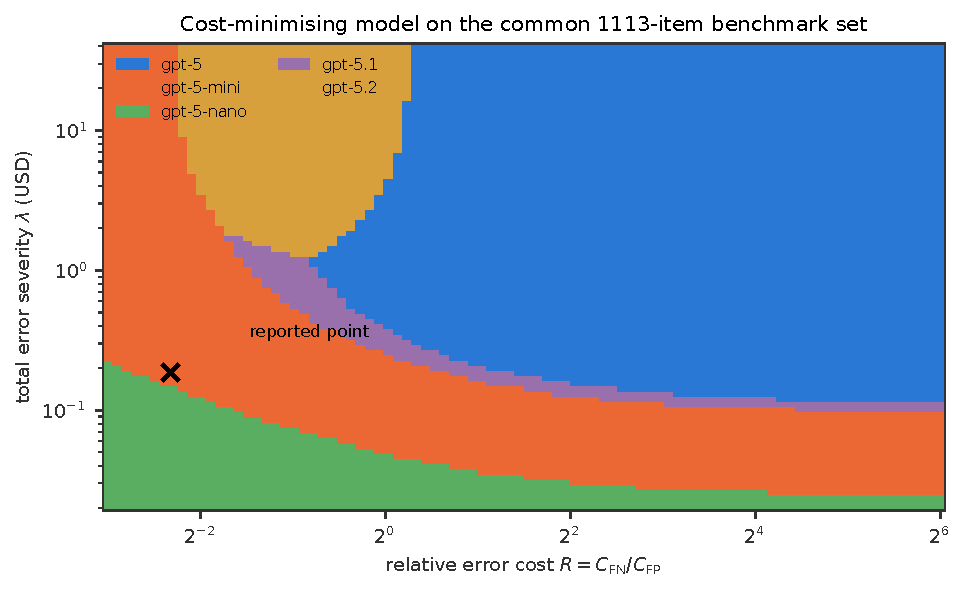
\includegraphics[width=0.9\linewidth]{assets/evidence/fig_canonical_cost_decision_map.pdf}
    \caption[Cost-minimising model over error-cost assumptions]{Model minimising the empirical plug-in loss over relative false-negative cost \(w\) and total error severity \(\lambda\). The cross marks the operating point reported in Table~\ref{tab:canonical-cost-comparison}. Large regions with different winners show why the result is conditional on declared penalties.}
    \label{fig:canonical-cost-decision-map}
\end{figure}
\provline{P5}

At the declared operating point, \texttt{gpt-5-mini} beats \texttt{gpt-5-nano} by only \(2.52\times10^{-4}\) USD per request. The margin is therefore small, and a modest change in the assumed penalties can change the winner. 


\chapter{Conclusion}
\label{chap:conclusion}

This thesis separates three decisions that are often conflated:
\begin{itemize}
    \item whether a black-box classifier changed on a fixed sensitivity set;
    \item whether the observation warrants investigation;
    \item which candidate is preferable for a stated business scenario.
\end{itemize}

\paragraph{RQ1: How can campaign-relevance classification by an external LLM API be formalised as repeated evaluation of a non-stationary black-box binary classifier?}
Campaign-relevance classification by an external LLM API can be formalised as repeated evaluation of a non-stationary black-box binary classifier on fixed labelled items. The observable object is the binary output produced under a fixed client-controlled request contract, while the provider-side state remains hidden. This makes it possible to separate three roles clearly: the production task, the full benchmark used for broad comparison, and the frozen monitoring panel used for repeated paired checks. The same frozen items admit a newly released model into that comparison as soon as a first eligible run exists; that run is the model's baseline for later paired checks. Intentional prompt changes remain conceptually separate from passive behavioural drift.

\paragraph{RQ2: How can a reduced monitoring subset be constructed and sized so that routine evaluation is substantially cheaper while retaining sensitivity to behavioural change?}
The 300-item disagreement-enriched panel is a cheap fixed sensitivity set for routine monitoring. It is suitable for pairing the same posts across dates. Its construction concentrates evaluation effort on difficult cases, and the exact power analysis validates \(n=300\) as an adequate implemented size for the intended warning-panel role under the stated planning model, with \(\operatorname{Power}(300)\approx 0.80\). The panel is a low-cost warning instrument. Production-accuracy estimation is out of scope.

\paragraph{RQ3: Which paired statistical test and multiplicity treatment provide an appropriate rule for detecting directional degradation across repeated runs?}
The exact one-sided McNemar test is appropriate because the same labelled posts are observed in both runs. Its input is the imbalance between correct-to-wrong and wrong-to-correct transitions, not two independent accuracy estimates. Among 173 retrospective baseline-to-later comparisons, global Holm correction left one alert: \texttt{gpt-4.1-mini} declined by 12.5 percentage points from 15 to 22~March 2026 (\(n=296\), \(b=49\), \(c=12\), \(p_{\mathrm{Holm}}=1.704\times10^{-4}\)). It recovered in the next run. This is an observed temporary correctness change on the panel.

\paragraph{RQ4: How should candidate models be compared and selected when predictive quality, inference cost, and campaign-specific false-positive and false-negative costs differ?}
On 1,113 common full-benchmark cases, candidates can be compared by mean inference charge plus weighted false-positive and false-negative counts. At the illustrative penalty point \(C_{\mathrm{FP}}=0.155\) USD and \(C_{\mathrm{FN}}=0.031\) USD, \texttt{gpt-5-mini} has loss \(0.003697\), narrowly below \texttt{gpt-5-nano} at \(0.003779\). The ranking depends on both relative and absolute error costs, so a different business scenario can select a different model.

\section{Contribution and limits}

The contribution is a concrete decision pipeline:
\begin{itemize}
    \item a fixed client-controlled request contract and stable item identifiers make repeated pairing possible;
    \item a disagreement-enriched panel reduces monitoring cost;
    \item the frozen labelled items admit a newly released model into the same comparison as existing candidates, with its first eligible run serving as the baseline for later paired checks;
    \item exact paired testing with retrospective Holm correction controls the stated decision family;
    \item manual review separates an alert from an action;
    \item the full benchmark supports scenario-specific candidate selection.
\end{itemize}

The main limits are material:
\begin{itemize}
    \item the panel is a disagreement-enriched sensitivity set;
    \item the original disagreement-selection matrix is unavailable for exact replay;
    \item the stored manifest lacks immutable request hashes;
    \item the error prices are scenario inputs.
\end{itemize}
Future work should:
\begin{itemize}
    \item compare random and disagreement-enriched panels prospectively;
    \item pre-register an online multiple-testing rule;
    \item preserve immutable evaluation artifacts;
    \item estimate penalties from real business outcomes.
\end{itemize}

The recorded episode shows why this separation is useful: an observed alert can be real, temporary, and irrelevant to the deployed model. The correct response was review and continued monitoring.


\appendix
\chapter{Supplementary Tables}
\label{app:supplementary-tables}

\section{Batch Pricing Table}
\label{app:batch-pricing-table}

\begin{table}[htbp]
    \centering
    \caption{Batch-API prices per one million tokens (USD) for all models in \texttt{config/models.yaml} as of 16~March~2026.}
    \label{tab:batch-pricing-examples}
    \begin{tabular}{lll}
        \toprule
        Model & Input price & Output price \\
        \midrule
        \texttt{gpt-5.4-2026-03-05}      & 1.25  & 7.50  \\
        \texttt{gpt-5.4}                 & 1.25  & 7.50  \\
        \texttt{gpt-5.2}                 & 0.875 & 7.00  \\
        \texttt{gpt-5.2-pro}             & 10.50 & 84.00 \\
        \texttt{gpt-5.1}                 & 0.625 & 5.00  \\
        \texttt{gpt-5}                   & 0.625 & 5.00  \\
        \texttt{gpt-5-pro}               & 7.50  & 60.00 \\
        \texttt{gpt-5-mini}              & 0.125 & 1.00  \\
        \texttt{gpt-5-nano}              & 0.025 & 0.20  \\
        \texttt{gpt-4.1}                 & 1.00  & 4.00  \\
        \texttt{gpt-4.1-mini}            & 0.20  & 0.80  \\
        \texttt{gpt-4.1-nano}            & 0.05  & 0.20  \\
        \texttt{gpt-4o-2024-05-13}       & 2.50  & 7.50  \\
        \texttt{gpt-4o}                  & 1.25  & 5.00  \\
        \texttt{gpt-4o-mini}             & 0.075 & 0.30  \\
        \texttt{o1}                      & 7.50  & 30.00 \\
        \texttt{o1-pro}                  & 75.00 & 300.00 \\
        \texttt{o1-mini}                 & 0.55  & 2.20  \\
        \texttt{o3}                      & 1.00  & 4.00  \\
        \texttt{o3-pro}                  & 10.00 & 40.00 \\
        \texttt{o3-mini}                 & 0.55  & 2.20  \\
        \texttt{o3-deep-research}        & 5.00  & 20.00 \\
        \texttt{o4-mini}                 & 0.55  & 2.20  \\
        \texttt{o4-mini-deep-research}   & 1.00  & 4.00  \\
        \texttt{gemini-3-flash-preview}           & 0.25  & 1.50  \\
        \texttt{gemini-2.5-flash}                 & 0.15  & 1.25  \\
        \texttt{gemini-2.5-flash-preview-09-2025} & 0.15  & 1.25  \\
        \texttt{gemini-2.0-flash}                 & 0.05  & 0.20  \\
        \texttt{gemini-2.5-pro}                   & 0.625 & 5.00  \\
        \texttt{claude-opus-4-6}   & 2.97 & 14.88 \\
        \texttt{claude-opus-4-5}   & 2.97 & 14.88 \\
        \texttt{claude-opus-4-1}   & 8.92 & 44.63 \\
        \texttt{claude-opus-4}     & 8.92 & 44.63 \\
        \texttt{claude-sonnet-4-6} & 1.78 & 8.92  \\
        \texttt{claude-sonnet-4-5} & 1.78 & 8.92  \\
        \texttt{claude-sonnet-4}   & 1.78 & 8.92  \\
        \texttt{claude-haiku-4-5}  & 0.59 & 2.97  \\
        \texttt{claude-3.5-haiku}  & 0.40 & 2.00  \\
        \bottomrule
    \end{tabular}
\end{table}

\section{Per-metric ranking charts (monitoring snapshot)}
\label{app:per-metric-ranking-charts}

The following charts are supplementary visualizations of the exported monitoring snapshot from \texttt{assets/metrics\_export/}. They complement, but do not replace, the main decision tables in Chapters~\ref{ch:cost-deployment-utility} and~\ref{chap:system-architecture}.
Formal metric definitions and formulas are given in Chapter~\ref{ch:drift} (Section~\ref{sec:classification-metrics}); interpretation of metric movement for operational decisions is provided in Chapter~\ref{chap:system-architecture} and the episode narrative in Chapter~\ref{chap:degradation-case-study}.

\IfFileExists{assets/fig-metric-accuracy.png}{%
\begin{figure}[htbp]
    \centering
    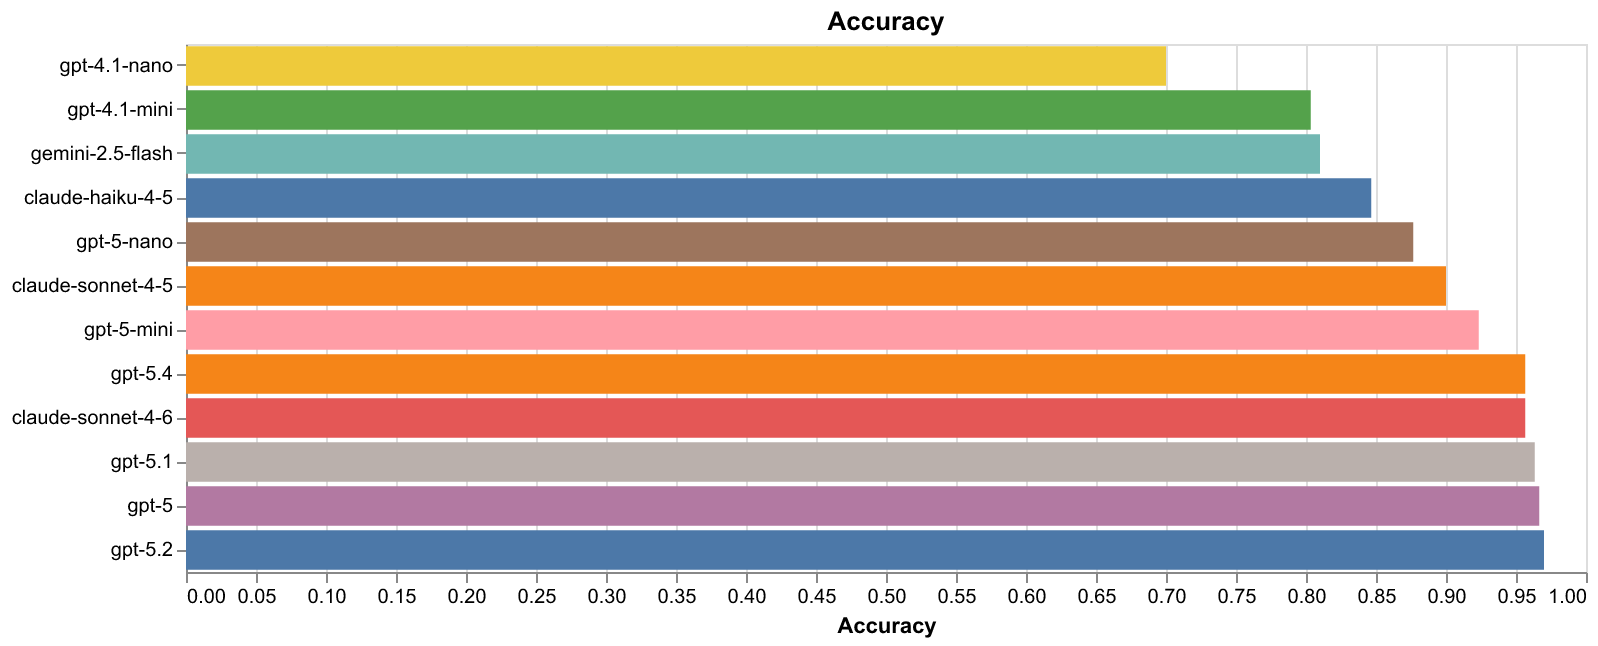
\includegraphics[width=\linewidth]{assets/fig-metric-accuracy.png}
    \caption{Per-model ranking by accuracy on $\mathcal{D}_n$.}
\end{figure}
}{}

\IfFileExists{assets/fig-metric-balanced_accuracy.png}{%
\begin{figure}[htbp]
    \centering
    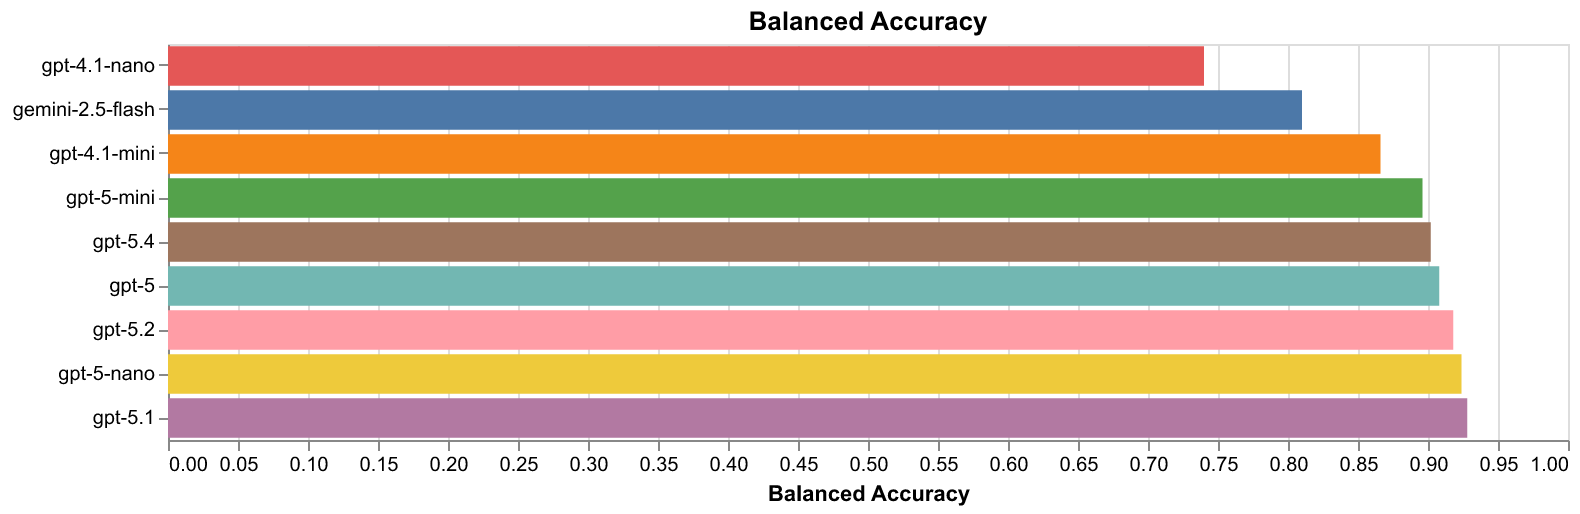
\includegraphics[width=\linewidth]{assets/fig-metric-balanced_accuracy.png}
    \caption{Per-model ranking by balanced accuracy on $\mathcal{D}_n$.}
\end{figure}
}{}

\IfFileExists{assets/fig-metric-f1.png}{%
\begin{figure}[htbp]
    \centering
    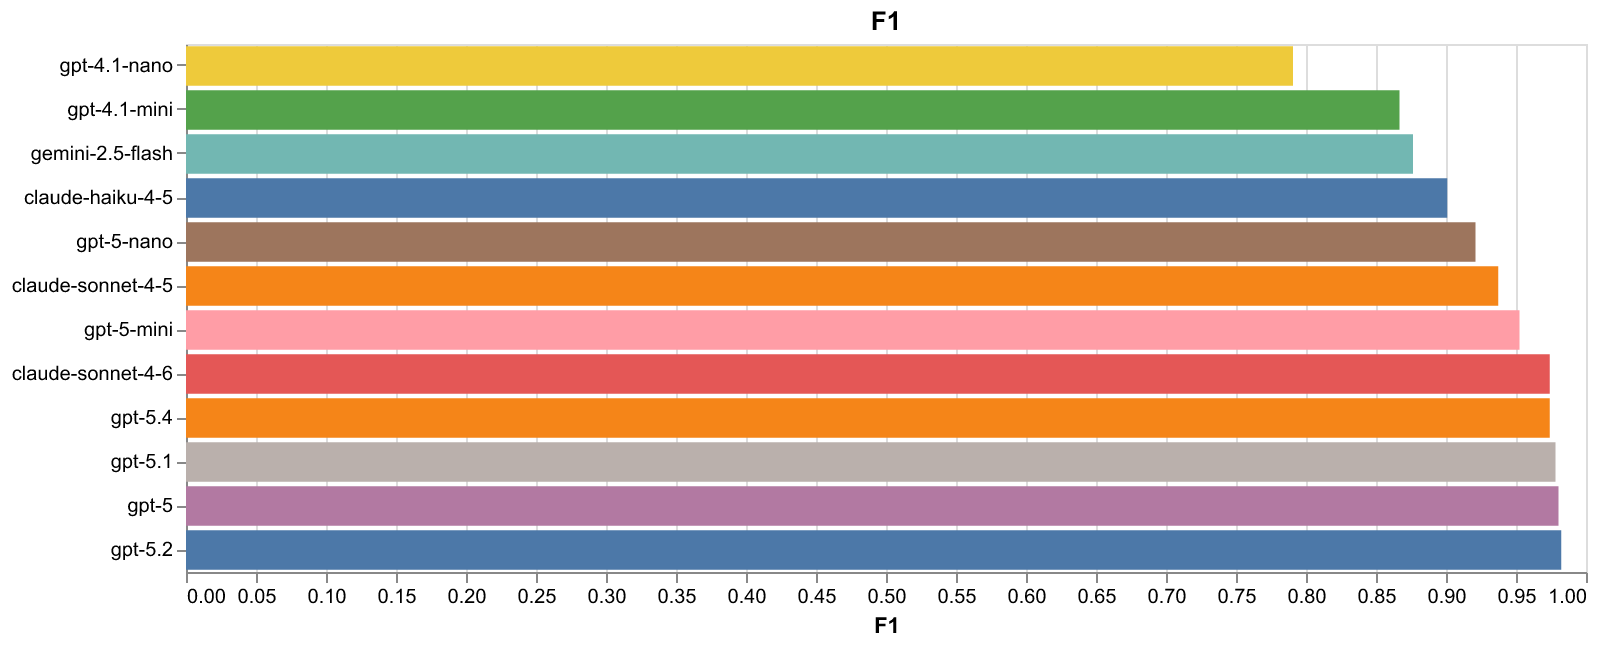
\includegraphics[width=\linewidth]{assets/fig-metric-f1.png}
    \caption{Per-model ranking by F1 score on $\mathcal{D}_n$.}
\end{figure}
}{}

\IfFileExists{assets/fig-metric-pr_auc.png}{%
\begin{figure}[htbp]
    \centering
    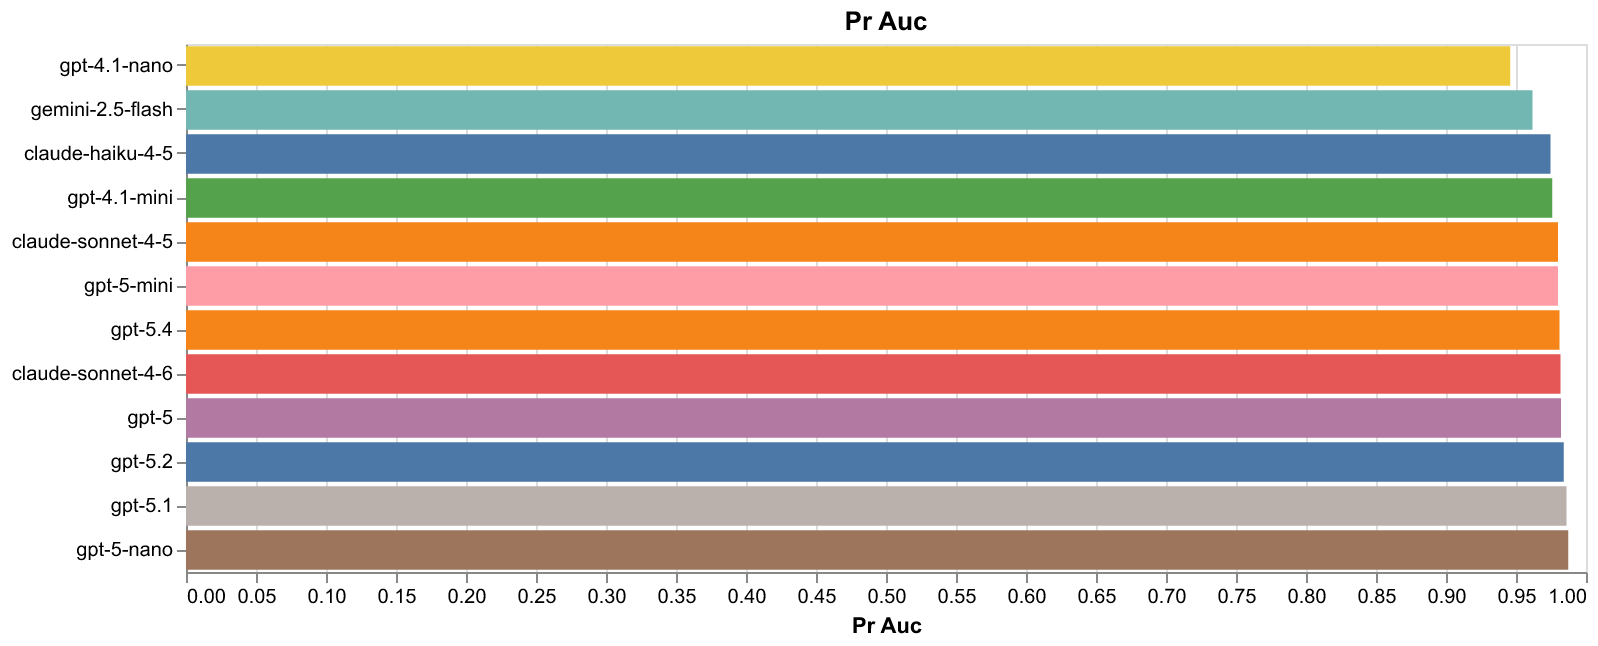
\includegraphics[width=\linewidth]{assets/fig-metric-pr_auc.png}
    \caption{Per-model ranking by PR--AUC on $\mathcal{D}_n$.}
\end{figure}
}{}

\IfFileExists{assets/fig-metric-precision.png}{%
\begin{figure}[htbp]
    \centering
    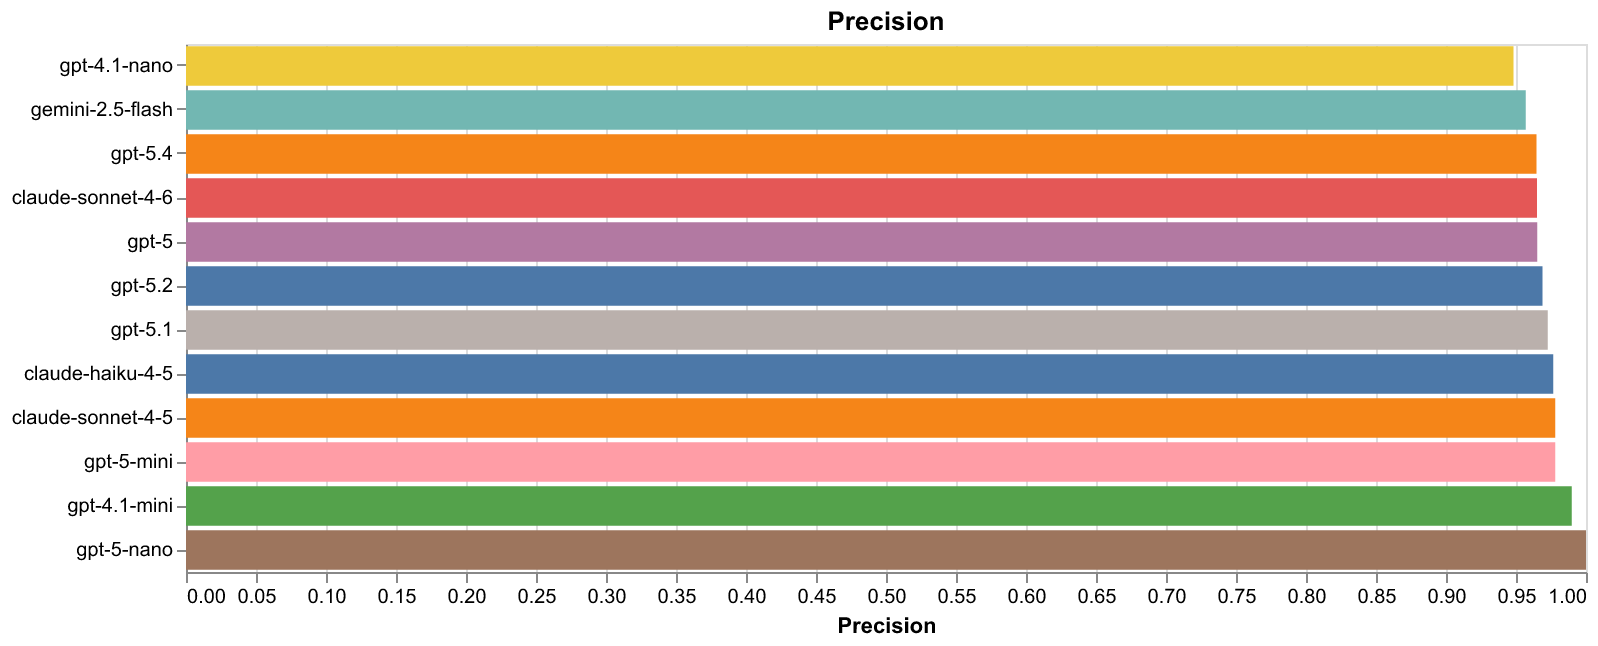
\includegraphics[width=\linewidth]{assets/fig-metric-precision.png}
    \caption{Per-model ranking by precision on $\mathcal{D}_n$.}
\end{figure}
}{}

\IfFileExists{assets/fig-metric-recall.png}{%
\begin{figure}[htbp]
    \centering
    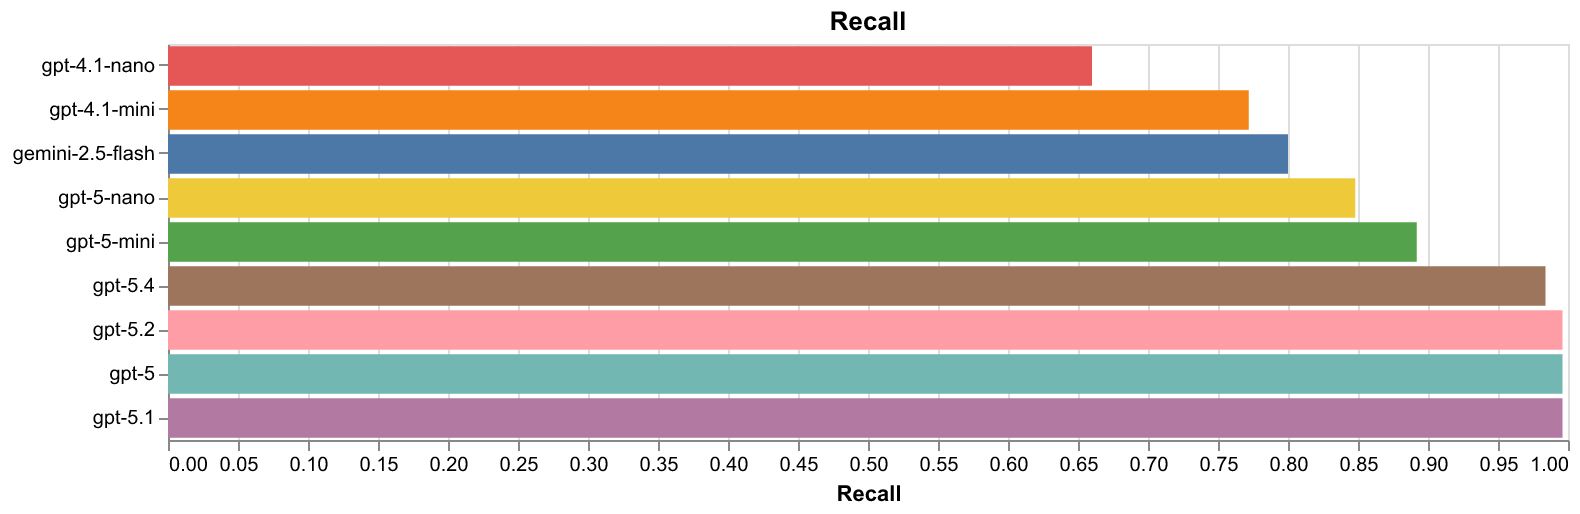
\includegraphics[width=\linewidth]{assets/fig-metric-recall.png}
    \caption{Per-model ranking by recall on $\mathcal{D}_n$.}
\end{figure}
}{}

\IfFileExists{assets/fig-metric-specificity.png}{%
\begin{figure}[htbp]
    \centering
    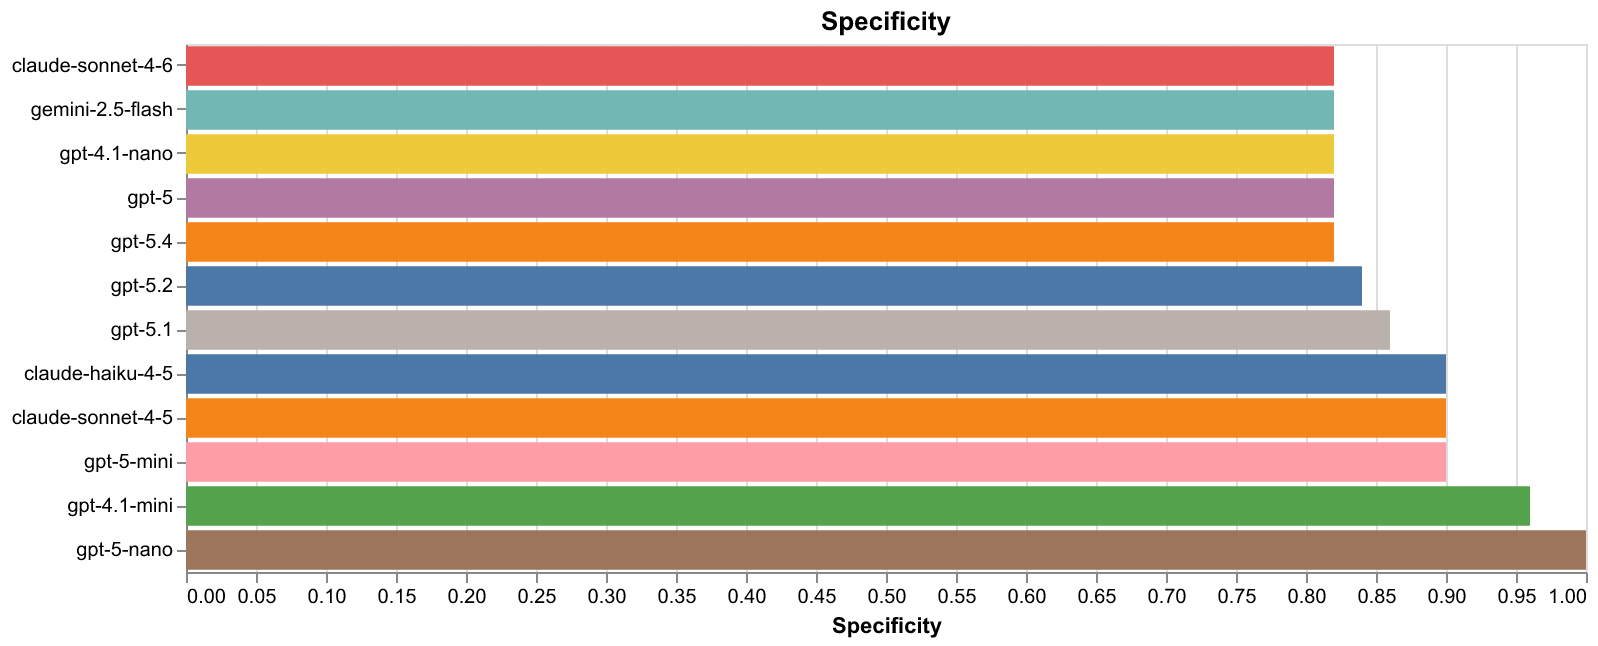
\includegraphics[width=\linewidth]{assets/fig-metric-specificity.png}
    \caption{Per-model ranking by specificity on $\mathcal{D}_n$.}
\end{figure}
}{}



{}



\end{document}
